%%%%%%%%%%%%%%%%%%%%%%%%%%%%%%%%%%%%%%%%%%%%%%%%%%%%%%%%%%%%
\documentclass[a4paper,11pt,oneside]{article}
\usepackage[a4paper,vmargin={1.5cm,1.5cm},width=16cm]{geometry}
\usepackage[style=verbose-inote,doi=false,sortcites=true,block=space,backend=bibtex]{biblatex}
\usepackage[utf8]{inputenc}
\usepackage{textcomp}
\usepackage[spanish]{babel}
\usepackage{microtype}
\usepackage{lmodern}
\usepackage{graphicx}
\usepackage{fancyhdr}
\usepackage{booktabs}
\usepackage{eurosym}
\usepackage{mathptmx}
\usepackage[T1]{fontenc}
\usepackage{hyperref}
%% Added to help mimic structure.
\usepackage{tcolorbox}
\usepackage{soul}
\usepackage{color}
\usepackage{lastpage}
%%%%%%%%%%%%%%%%%%%%%%%%%%%%%%%%%%%%%%%%%%%%%%%%%%%%%%%%%%%%
%% HEADERS
%\setlength{\headheight}{1cm}
%\setlength{\headsep}{0.5cm}
%\pagestyle{fancyplain}
%\fancyhf{}
%\lhead{\fancyplain{}{\sc Memoria científico técnica de proyectos coordinados}}
%\rhead{\fancyplain{}{\sc Parte A}}
%\cfoot{\thepage}
%\renewcommand{\headrulewidth}{0pt} % remove lines
%\renewcommand{\footrulewidth}{0pt}


%%% HEADER
\setlength{\headheight}{1cm}
%\setlength{\headwidth}{20cm}
\setlength{\headsep}{0.5cm}
\pagestyle{fancyplain}
\fancyheadoffset[HR,HL]{2cm}
\fancyhf{}
\lhead{\raisebox{-0.4\height}{
\includegraphics[height=0.9cm,keepaspectratio=true]{img/miniLogo}}}
\rhead{\fancyplain{}{\fontsize{10}{12} \selectfont \textbf{\underline{Memoria científico técnica de proyectos coordinados}}}}
\cfoot{\thepage\, / parte A}
\renewcommand{\headrulewidth}{0pt} % remove lines
\renewcommand{\footrulewidth}{0pt}
%%%%%%%%%%%%%%%%%%%%%%%%%%%%%%%%%%%%%%%%%%%%%%%%%%%%%%%%%%%%
%% Hack to make math formulas bold in section titles
\makeatletter
\DeclareRobustCommand*{\bfseries}{%
  \not@math@alphabet\bfseries\mathbf
  \fontseries\bfdefault\selectfont
  \boldmath
}
\makeatother

%%%%%%%%%%%%%%%%%%%%%%%%%%%%%%%%%%%%%%%%%%%%%%%%%%%%%%%%%%%%
\def\thesection{\bf \textsf{\Alph{section}}}

%\nobibliography{biblio}
%\bibliographystyle{JHEP}

\bibliography{biblio}


%%%%%%%%%%%%%%%%%%%%%%%%%%%%%%%%%%%%%%%%%%%%%%%%%%%%%%%%%%%%
\begin{document}

%% Some useful definitions
% BB
\newcommand{\bb}{\ensuremath{\beta\beta}}
% BB0NU
\newcommand{\bbonu}{\ensuremath{\beta\beta0\nu}}
% BB2NU
\newcommand{\bbtnu}{\ensuremath{\beta\beta2\nu}}
% NME
\newcommand{\Monu}{\ensuremath{\Big|M_{0\nu}\Big|}}
\newcommand{\Mtnu}{\ensuremath{\Big|M_{2\nu}\Big|}}
% PHASE-SPACE FACTOR
\newcommand{\Gonu}{\ensuremath{G_{0\nu}(\Qbb, Z)}}
\newcommand{\Gtnu}{\ensuremath{G_{2\nu}(\Qbb, Z)}}

% mbb
\newcommand{\mbb}{\ensuremath{m_{\beta\beta}}}
\newcommand{\kgy}{\ensuremath{\rm kg \cdot y}}
\newcommand{\ckky}{\ensuremath{\rm counts/(keV \cdot kg \cdot y)}}
\newcommand{\mbba}{\ensuremath{m_{\beta\beta}^a}}
\newcommand{\mbbb}{\ensuremath{m_{\beta\beta}^b}}
\newcommand{\mbbt}{\ensuremath{m_{\beta\beta}^t}}
\newcommand{\nbb}{\ensuremath{N_{\beta\beta^{0\nu}}}}

% Qbb
\newcommand{\Qbb}{\ensuremath{Q_{\beta\beta}}}

% Tonu
\newcommand{\Tonu}{\ensuremath{T_{1/2}^{0\nu}}}

% Tonu
\newcommand{\Ttnu}{\ensuremath{T_{1/2}^{2\nu}}}

% Xe-136
\newcommand{\Xe}{\ensuremath{^{136}}Xe}

% Xe-136
\newcommand{\CS}{\ensuremath{^{137}}Cs}

% Xe-136
\newcommand{\NA}{\ensuremath{^{22}}Na}


% Bi-214
\newcommand{\Bi}{\ensuremath{^{214}}Bi}

% Tl-208
\newcommand{\Tl}{\ensuremath{^{208}}Tl}

% Pb-208
\newcommand{\Pb}{\ensuremath{^{208}}Pb}
% Pb-208
\newcommand{\PBD}{\ensuremath{^{210}}Pb}

% Po-214
\newcommand{\Po}{\ensuremath{^{214}}Po}

% bru
\newcommand{\bru}{cts/(keV$\cdot$kg$\cdot$y)}

% Saltos de carro en tablas
\newcommand{\minitab}[2][l]{\begin{tabular}{#1}#2\end{tabular}}

\newcommand{\thedraft}{0.1.1}% version for referees

\newcommand{\MO}{\ensuremath{{}^{100}{\rm Mo}}}
\newcommand{\SE}{\ensuremath{{}^{82}{\rm Se}}}
\newcommand{\ZR}{\ensuremath{{}^{96}{\rm Zr}}}
\newcommand{\KR}{\ensuremath{{}^{82}{\rm Kr}}}
\newcommand{\ND}{\ensuremath{{}^{150}{\rm Nd}}}
\newcommand{\XE}{\ensuremath{{}^{136}\rm Xe}}
\newcommand{\GE}{\ensuremath{{}^{76}\rm Ge}}
\newcommand{\GES}{\ensuremath{{}^{68}\rm Ge}}
\newcommand{\TE}{\ensuremath{{}^{128}\rm Te}}
\newcommand{\TEX}{\ensuremath{{}^{130}\rm Te}}
\newcommand{\TL}{\ensuremath{{}^{208}\rm{Tl}}}
\newcommand{\CA}{\ensuremath{{}^{48}\rm Ca}}
\newcommand{\CO}{\ensuremath{{}^{60}\rm Co}}
\newcommand{\PO}{\ensuremath{{}^{214\rm Po}}}
\newcommand{\U}{\ensuremath{{}^{235}\rm U}}
\newcommand{\CT}{\ensuremath{{}^{10}\rm C}}
\newcommand{\BE}{\ensuremath{{}^{11}\rm Be}}
\newcommand{\BO}{\ensuremath{{}^{8}\rm Be}}
\newcommand{\UDTO}{\ensuremath{{}^{238}\rm U}}
\newcommand{\CD}{\ensuremath{^{116}{\rm Cd}}}
\newcommand{\THO}{\ensuremath{{}^{232}{\rm Th}}}
\newcommand{\BI}{\ensuremath{{}^{214}}Bi}


%% Heading
\begin{tcolorbox}[colback=white,arc=0pt,outer arc=0pt,colframe=black,boxrule=0.6pt]
\begin{center}
Convocatorias 2014\\ 
Proyectos de I+D ``Excelencia'' y Proyectos de I+D+I ``Retos Investigación" \\ 
Dirección General de Investigación Científica y Técnica \\
Subdirección General de Proyectos de Investigación
\end{center} 
\end{tcolorbox}

\begin{tcolorbox}[colback=yellow,arc=0pt,outer arc=0pt,colframe=black,boxrule=0.6pt,left=0mm,right=0mm]
  \begin{center}
    AVISO IMPORTANTE\\
  \end{center}
    En virtud del art\'iculo 11 de la convocatoria \ul{\textbf{NO SE ACEPTAR\'AN NI SER\'AN SUBSABABLES MEMORIAS CIENT\'IFICO-T\'ECNICAS}} que no se presenten en este formato.\\
    \\
    \textbf{Lea detenidamente las instrucciones que figuran al final de este documento para rellenar correctamente la memoria cient\'ifico-t\'ecnica.}
    \\
  %\end{center}
\end{tcolorbox}
\vspace{3pt}
\begin{tcolorbox}[colback=yellow,arc=0pt,outer arc=0pt,colframe=black,boxrule=0.6pt,left=0mm]
  \noindent\textbf{Parte A: RESUMEN DE LA PROPUESTA/SUMMARY OF THE PROPOSAL}
  %\section{RESUMEN DE LA PROPUESTA/SUMMARY OF THE PROPOSAL}
\end{tcolorbox}

%%%%%%%%%%%%%%%%%%%%%%%%%%%%%%%%%%%%%%%%%%%%%%%%%%%%%%%%%%%%%%%%%%%%%%%%%%%%%

%\section{RESUMEN DE LA PROPUESTA/SUMMARY OF THE PROPOSAL}

%%%%%%%%%%%%%%%%%%%%%%%%%%%%%%%%%%%%%%%%%%%%%%%%%%%%%%%%%%%%%%%%%%%%%%%%%%%%%

%\subsection{DATOS DEL PROYECTO COORDINADO}
\noindent\textbf{A.1. DATOS DEL PROYECTO COORDINADO}
\vspace{6pt}

\noindent\textbf{INVESTIGADOR COORDINADOR PRINCIPAL 1:} (Nombre y apellidos)

\noindent Juan José Gómez Cadenas.
\vspace{6pt}

\noindent\textbf{INVESTIGADOR COORDINADOR PRINCIPAL 2:} (Nombre y apellidos)

\noindent Michel Sorel
\vspace{6pt}

\noindent\textbf{TÍTULO GENERAL DEL PROYECTO COORDINADO:} Construcción operación e I+D+i para el experimento NEXT en el LSC.
\vspace{6pt}

\noindent\textbf{ACRÓNIMO DEL PROYECTO COORDINADO:} NEXT.


\noindent\textbf{RESUMEN DEL PROYECTO COORDINADO} 
{\color{blue}{M\'aximo 3500 caracteres (incluyendo espacios en blanco):}}
\vspace{12pt}

%%

NEXT (Neutrino Experiment with a Xenon TPC) es un experimento para buscar desintegraciones doble beta sin neutrinos (\bbonu), cuya detección demostraría unívocamente que el neutrino es una partícula de Majorana (es decir su propia antipartícula) y supondría un descubrimiento con profundas consecuencias en física de partículas y cosmología. 

 El isótopo escogido por NEXT es el \XE. El experimento dispone de cien kilos de gas xenón enriquecido al 90\% en \XE. La tecnología se basa en el uso de cámaras de proyección temporal operando a una presión típica de 15 atmósferas (\HPXE). Las características principales de esta técnica experimental son: a) excelente resolución en la medida de la energía; b) capacidad de reconstruir la trayectoria de los electrones emitidos en la desintegración, lo que refuerza la capacidad del experimento para reducir el ruido de fondo; c) escalabilidad a grandes masa y d) la posibilidad de reducir el ruido de fondo hasta niveles despreciables mediante la técnica conocida como \BATA\ (de las siglas en inglés, {\em Barium Tagging}).

 El experimento NEXT contempla cuatro fases: i) Demostración de la tecnología \HPXE\ con prototipos que usan $\sim$1 kg de xenón natural; ii) Medida de los ruidos de fondo y de la señal del proceso permitido (\bbtnu) con un detector (NEW) basado en 12 kilos de xenón enriquecido y operando en el Laboratorio Subterráneo de Canfranc (LSC); iii) Búsqueda de desintegraciones \bbonu\ con el detector NEXT-100, una réplica a escala 2:1 (en tamaño) y 8:1 (en masa) de NEW, que usará por tanto 100 kilos de gas enriquecido; iv) Búsqueda de desintegraciones \bbonu\ con el detector BEXT (Barium-tagging Experiment with a Xenon TPC), con una masa de alrededor de una tonelada de \XE, que introducirá la técnica de \BATA\ para reducir el ruido de fondo hasta niveles despreciables. 

La primera fase de NEXT ha sido completada con éxito durante el periodo 2009-2013. Durante esta etapa se han construido los prototipos NEXT-DEMO (IFIC) y NEXT-DBDM (Berkeley) que han demostrado las características principales de la tecnología. El experimento se encuentra en estos momentos en su segunda fase. El detector NEW está siendo construido por la colaboración y operará en el LSC durante el año 2015. La financiación del detector NEW proviene de un Advanced Grant (AdG/ERC) concedido en 2013 al IP de este proyecto (operativo desde Febrero de 2014 a Febrero de 2018). El detector NEXT-100 supone la tercera fase del proyecto. Se construirá y pondrá a punto durante 2016 y 2017 e iniciará su toma de datos en 2018. La cuarta fase depende de los resultados de la fase tres, en la que se podría realizar ya un descubrimiento. Previsiblemente, BEXT podría funcionar en el LSC a partir del 2020. 

 NEXT es  una colaboración internacional, liderada por grupos españoles y con una fuerte contribución de grupos norteamericanos. El desarrollo de la tecnología laser necesaria para el BaTa se realiza en colaboración con el Centro de Láseres Pulsados de Salamanca (CLPU). 

 Este  proyecto de investigación requiere {\em cofinanciación} para desarrollar la fase tres del experimento. Concretamente, se requiere: a) fondos para adquirir una parte de los equipos y material fungible necesarios para la construcción del detector NEXT-100 (cofinanciado por el AdG y los fondos provenientes de la colaboración); b) fondos para una parte del personal científico y técnico; y c) fondos para cofinanciar el R\&D dedicado al \BATA.  

 
\vspace{12pt}

\noindent\textbf{PALABRAS CLAVE DEL PROYECTO COORDINADO:} neutrinos, TPC, HPXe, xenón, desintegración doble beta, Canfranc, alta presión, electroluminescencia. 

\vspace{12pt}

\noindent\textbf{TITLE OF THE COORDINATED PROJECT:} Construction operation and R\&D for the NEXT experiment at the LSC. 
\vspace{6pt}

\noindent\textbf{ACRONYM OF THE COORDINATED PROJECT:} NEXT.
\vspace{6pt}

\noindent\textbf{SUMMARY OF THE COORDINATED PROJECT} 
\vspace{6pt}

%%

NEXT (Neutrino Experiment with a Xenon TPC) is an experiment to search neutrino less double beta decay processes (\bbonu). The detection of such processes would demonstrate that neutrinos are Majorana particles (that is their own antiparticles) and would have deep consequences in physics and cosmology.  

The isotope chosen by NEXT is  \XE. The collaboration has access to hundred kilograms of xenon enriched at 90\% in \XE, owned by the Underground Laboratory of Canfranc (LSC). The NEXT technology is based in the use of time projection chambers operating at a typical pressure of 15 bar and using electroluminescence to amplify the signal (\HPXE). The main advantages of the experimental technique are: a) excellent energy resolution; b) the ability to reconstruct the trajectory of the two electrons emitted in the decays, a unique feature of the \HPXE\ which further contributes to the suppression of backgrounds; c) scalability to large masses; and d) the possibility to reduce the background to negligible levels thanks to the barium tagging technology (\BATA).

The NEXT roadmap was designed in four stages: i) Demonstration of the \HPXE\ technology with prototypes deploying a mass of natural xenon in the range of 1 kg; ii) Characterisation of the backgrounds to the \bbonu\ signal and measurement of the \bbtnu\ signal with the NEW detector, deploying 12 kg of enriched xenon and operating at the LSC; iii) Search for \bbonu\ decays with the NEXT-100 detector, which scales up the NEW detector by a factor 2:1 in size (8:1 in mass) and deploys, thus, 100 kg of enriched xenon. iv) Search for \bbonu\ decays with the BEXT detector (Barium-tagging Experiment with a Xenon TPC), which will deploy a mass in the ton scale and will introduce the technology of \BATA\ in order to reduce backgrounds to negligible levels.  

The first stage of NEXT has been successfully completed during the period 2009-2013. The prototypes NEXT-DEMO (IFIC) and NEXT-DBDM (Berkeley) were built and operated for more than two years. These apparatus have demonstrated the main features of the technology. The experiment is currently developing its second phase. The NEW detector is being constructed during 2014 and will operate in the LSC during 2015. The funding for the construction and operation of NEW comes from an Advanced Grant (AdG/ERC) granted to the PI of this project in 2013. The NEXT-100 detector will be built and commissioned during 2016 and 2017 and will start data taking in 2018. NEXT-100 could discover \bbonu\ processes if the period of the decay is equal or less than $6 \times 10^{25}$~year. The fourth phase of the experiment (BEXT) could start in 2020. 

NEXT is an international collaboration, lead by spanish groups (the PI of this proposal is the spokesperson of the collaboration) and with a very significant contribution of US groups. The laser technology needed for the BEXT phase is being developed in collaboration with the spanish Center for Pulsed Lasers (CLPU). 

 This proposal requires {\em co-funding} to complete the phase three of the experiment. Specifically we request: a) funds to co-finance the construction of the NEXT-100 detector (which is being partially funded by the AdG as well as by the international collaboration, primarily US groups); b) funds to co-finance personnel; and c) a  contribution of the R\&D to develop the \BATA\ technology.   



 \vspace{12pt}

\noindent\textbf{KEYWORDS OF THE COORDINATED PROJECT:} neutrinos, TPC, HPXe, xenon, double beta decay, Canfranc, high pressure, electroluminescence. 

 \vspace{12pt}
%\newpage

%%%%%%%%%%%%%%%%%%%%%%%%%%%%%%%%%%%%%%%%%%%%%%%%%%%%%%%%%%%%%%%%%%%%%%%%%%%%%

\noindent\textbf{A.2. DATOS DE LOS SUBPROYECTOS/ DATA OF SUBPROJECTS }
 \vspace{12pt}
 
\noindent\textbf{SUBPROYECTO 1 / SUBPROJECT 1} (el investigador o investigadores principales son los coordinadores del proyecto coordinado)

\vspace{6pt}
\noindent\textbf{TÍTULO / TITLE :} Coordination of the NEXT project (COORD)
%
%\begin{itemize}
%\item {\bf IP 1 / PI 1}: Juan José Gómez Cadenas (co-coordinator)
%\item {\bf IP 2 / PI 2}: Michel Sorel (co-coordinator)
%\item {\bf Título / Title}: Coordination of the NEXT project (COORD)
%\end{itemize}

 \vspace{12pt}
 
\noindent\textbf{SUBPROYECTO 2 / SUBPROJECT 2}
\vspace{6pt}

\noindent\textbf{INVESTIGADOR PRINCIPAL 1 / PRINCIPAL RESEARCHER 1 } (nombre y apellidos)

\vspace{6pt}
\noindent Jos\'e F. Toledo

\vspace{12pt}
\noindent\textbf{INVESTIGADOR PRINCIPAL 2 / PRINCIPAL RESEARCHER 2} (nombre y apellidos)

\vspace{6pt}
\noindent Ra\'ul Esteve

\vspace{6pt}
\noindent\textbf{TÍTULO / TITLE :} Electronics and DAQ for NEXT

\vspace{12pt}
\noindent\textbf{SUBPROYECTO 3 / SUBPROJECT 3}
\vspace{6pt}

\noindent\textbf{INVESTIGADOR PRINCIPAL 1 / PRINCIPAL RESEARCHER 1 } (nombre y apellidos)

\vspace{6pt}
\noindent José A. Hernando Morata

\vspace{6pt}
\noindent\textbf{TÍTULO / TITLE :} Calibration and Reconstruction for NEXT (CALREC)

\vspace{12pt}
\noindent\textbf{SUBPROYECTO 4 / SUBPROJECT 4}
\vspace{6pt}

\noindent\textbf{INVESTIGADOR PRINCIPAL 1 / PRINCIPAL RESEARCHER 1 } (nombre y apellidos)

\vspace{6pt}
\noindent Alicia Vázquez

\vspace{6pt}
\noindent\textbf{TÍTULO / TITLE :} Barium Tagging (BATA)


%\rhead{\fancyplain{}{\sc Parte B}}
%\newpage
%\setcounter{page}{1}

%%%%%%%%%%%%%%%%%%%%%%%%%%%%%%%%%%%%%%%%%%%%%%%%%%%%%%%%%%%%%%%%%%%%%%%%%%%%%
\newpage
\setcounter{page}{1}
\cfoot{\fancyplain{}{\thepage\, / parte B}}

%\section{INFORMACIÓN ESPECÍFICA DEL EQUIPO / TEAM INFORMATION}

\begin{tcolorbox}[colback=yellow,arc=0pt,outer arc=0pt,colframe=black,boxrule=0.6pt,left=0mm]
  \noindent\textbf{PARTE B: INFORMACIÓN ESPECÍFICA DEL EQUIPO / TEAM INFORMATION}
  %\section{RESUMEN DE LA PROPUESTA/SUMMARY OF THE PROPOSAL}
\end{tcolorbox}

\vspace{12pt}
\noindent\textbf{B.1 RELACIÓN DE LAS PERSONAS NO DOCTORES QUE COMPONEN EL EQUIPO DE TRABAJO / WORKING TEAM (MEMBERS WITHOUT PH.D) }
%B.1. RELACIÓN DE LAS PERSONAS NO DOCTORES QUE COMPONEN EL EQUIPO DE TRABAJO (se recuerda que los doctores del equipo de trabajo y los componentes del equipo de investigación no se solicitan aquí porque deberán incluirse en la aplicación informática de solicitud). Repita la siguiente secuencia tantas veces como precise para cada uno de los subproyectos.

%1. Nombre y apellidos: 
%Titulación: licenciado/ingeniero/graduado/máster/formación profesional/otros (especificar)
%Tipo de contrato: en formación/contratado/técnico/ entidad extranjera/otros (especificar)%
%Duración del contrato: indefinido/temporal
%Subproyecto al que pertenece (nombre y apellidos del investigador principal):

\begin{enumerate}
\item {\bf Nombre /Name}: David Lorca
\begin{itemize}
\item {\bf Titulación /Title}: Licenciado. 
\item {\bf Tipo de contrato /Contract type}: Formación/Training. 
\item {\bf Duración del contrato /Contract scope}: Temporal/Temporary. 
\item {\bf Subproyecto /Subproject}: COORD. 
\end{itemize}
\item {\bf Nombre /Name}: Ander Simó
\begin{itemize}
\item {\bf Titulación /Title}: Licenciado. 
\item {\bf Tipo de contrato /Contract type}: Formación/Training. 
\item {\bf Duración del contrato /Contract scope}: Temporal/Temporary. 
\item {\bf Subproyecto /Subproject}: COORD. 
\end{itemize}
\item {\bf Nombre /Name}: Luis Serra
\begin{itemize}
\item {\bf Titulación /Title}: Licenciado. 
\item {\bf Tipo de contrato /Contract type}: Formación/Training. 
\item {\bf Duración del contrato /Contract scope}: Temporal/Temporary. 
\item {\bf Subproyecto /Subproject}: COORD. 
\end{itemize}
\item {\bf Nombre /Name}: Miquel Nebot
\begin{itemize}
\item {\bf Titulación /Title}: Licenciado. 
\item {\bf Tipo de contrato /Contract type}: Formación/Training. 
\item {\bf Duración del contrato /Contract scope}: Temporal/Temporary. 
\item {\bf Subproyecto /Subproject}: COORD. 
\end{itemize}
\item {\bf Nombre /Name}: Vicente Álvarez
\begin{itemize}
\item {\bf Titulación /Title}: Ingeniero Técnico / Technical Engineer.  
\item {\bf Tipo de contrato /Contract type}: Técnico / Technical. 
\item {\bf Duración del contrato / Contract scope}: Temporal/Temporary. 
\item {\bf Subproyecto /Subproject}: COORD. 
\end{itemize}
\item {\bf Nombre /Name}: Marc Querol
\begin{itemize}
\item {\bf Titulación /Title}: Ingeniero Técnico / Technical Engineer.  
\item {\bf Tipo de contrato /Contract type}: Técnico / Technical. 
\item {\bf Duración del contrato / Contract scope}: Temporal/Temporary. 
\item {\bf Subproyecto /Subproject}: COORD. 
\end{itemize}
\item {\bf Nombre /Name}: Alberto Martínez
\begin{itemize}
\item {\bf Titulación /Title}: Ingeniero Técnico / Technical Engineer.  
\item {\bf Tipo de contrato /Contract type}: Técnico / Technical. 
\item {\bf Duración del contrato / Contract scope}: Temporal/Temporary. 
\item {\bf Subproyecto /Subproject}: COORD. 
\end{itemize}
\item {\bf Nombre /Name}: Gonzalo Mart\'inez Lema
\begin{itemize}
\item {\bf Titulación /Title}: Master en F\'isica de Part\'iculas / Master in Particle Physics.  
\item {\bf Tipo de contrato /Contract type}: Formación / Training. 
\item {\bf Duración del contrato / Contract scope}: Temporal/Temporary. 
\item {\bf Subproyecto /Subproject}: CALREC. 
\end{itemize}
\end{enumerate}


%%%%%%%%%%%%%%%%%%%%%%%%%%%%%%%%%%%%%%%%%%%%%%%%%%%%%%%%%%%%%%%%%%%%%%%%%%%%%

%\subsection{\label{subsec:Grants}FINANCIACIÓN PÚBLICA Y PRIVADA (PROYECTOS Y/O CONTRATOS DE I+D+I) DEL EQUIPO DE INVESTIGACIÓN / FUNDING OF RESEARCH TEAM}

\noindent\textbf{B.2 FINANCIACIÓN PÚBLICA Y PRIVADA (PROYECTOS Y/O CONTRATOS DE I+D+I) DEL EQUIPO DE INVESTIGACIÓN / FUNDING OF RESEARCH TEAM}
\vspace{12pt}
\noindent\textbf{SUBPROYECTO 1 / SUBPROJECT 1}

\begin{enumerate}
\item {\bf Investigadores / Researchers }: Juan José Gómez Cadenas, M. Sorel, I. Liubarsky, F. Monrabal, J.Martin-Albo, S. Cárcel, J. Rodríguez, N. López, J. Renner.
\begin{itemize}
\item {\bf Entidad financiadora / Funding Agency}: ERC. Advanced Grant 339787-NEXT 
\item {\bf Título / Title}:  NEXT.
\item {\bf Duración / Duration}: 01/02/2014 -- 31/01/2019. 
\item {\bf Financiación recibida / Grant}: 2.8 M\euro. 
\item {\bf Relación con el proyecto presentado / Relation with this subproject}: Mismo tema / Same topic. 
\item {\bf Estado del proyecto / Status of project}: Concedido / Granted
\item {\bf IP del proyecto / PI of project}: Juan José Gómez Cadenas
\end{itemize}
\item {\bf Investigadores / Researchers }: Juan José Gómez Cadenas, M. Sorel, I. Liubarsky, F. Monrabal, J.Martin-Albo, S. Cárcel, J. Rodríguez.
\begin{itemize}
\item {\bf Entidad financiadora / Funding Agency}: Ministerio de Educaci\'on y Ciencia, CSD2008-00037.
\item {\bf Título / Title}:  Canfranc Underground Physics (CUP).
\item {\bf Duración / Duration}: 15/12/2008 -- 15/12/2014. 
\item {\bf Financiación recibida / Grant}: 5.0 M\euro. 
\item {\bf Relación con el proyecto presentado / Relation with this subproject}: Mismo tema / Same topic. 
\item {\bf Estado del proyecto / Status of project}: Concedido / Granted
\item {\bf IP del proyecto / PI of project}: Concepción González-García 
\end{itemize}
\item {\bf Investigadores / Researchers }: Juan José Gómez Cadenas, M. Sorel, I. Liubarsky, F. Monrabal, J.Martin-Albo, S. Cárcel, J. Rodríguez.
\begin{itemize}
\item {\bf Entidad financiadora / Funding Agency}:  Ministerio de Econom\'ia y Competitividad, FIS2012-37947-C04-01.
\item {\bf Título / Title}:  Coordination of NEXT Project.
\item {\bf Duración / Duration}: 01/01/2013 -31/12/2014. 
\item {\bf Financiación recibida / Grant}:256,000\euro. 
\item {\bf Relación con el proyecto presentado / Relation with this subproject}: Mismo tema / Same topic. 
\item {\bf Estado del proyecto / Status of project}: Concedido / Granted
\item {\bf IP del proyecto / PI of project}: Juan José Gómez Cadenas 
\end{itemize}
\item {\bf Investigadores / Researchers }: Juan José Gómez Cadenas, M. Sorel.
\begin{itemize}
\item {\bf Entidad financiadora / Funding Agency}:  Ministerio de Educaci\'on y Ciencia, FPA2009-13697-C04-04
\item {\bf Título / Title}:  Física Experimental de Neutrinos en el IFIC / Experimental neutrino physics at IFIC
\item {\bf Duración / Duration}: 01/01/2010 -31/12/2012. 
\item {\bf Financiación recibida / Grant}:534,437\euro. 
\item {\bf Relación con el proyecto presentado / Relation with this subproject}: Muy relacionado / Very related. 
\item {\bf Estado del proyecto / Status of project}: Concedido / Granted
\item {\bf IP del proyecto / PI of project}: Juan José Gómez Cadenas 
\end{itemize}
\end{enumerate}

\vspace{12pt}

\noindent\textbf{SUBPROYECTO 2 / SUBPROJECT 2}

\begin{enumerate}
\item {\bf Investigador / Researcher }: R.Esteve Bosch, F.J.Mora Más, J.F. Toledo Alarcón
\begin{itemize}
\item {\bf Entidad financiadora / Funding Agency}: Ministerio de economía y competitividad: FIS2012-37947-C04-04.
\item {\bf Título / Title}:  Adquisición de datos y diseño mecánico para el experimento NEXT
\item {\bf Duración / Duration}: 01/01/2013 -31/12/2014
\item {\bf Financiación recibida / Grant}: 119.340 \euro. 
\item {\bf Relación con el proyecto presentado / Relation with this subproject}: Mismo tema / Same topic. 
\item {\bf Estado del proyecto / Status of project}: Concedido / Granted
\item {\bf IP del proyecto / PI of project}: J.F. Toledo Alarcón
\end{itemize}
\item {\bf Investigador / Researcher }: R.Esteve Bosch, F.J.Mora Más, J.F. Toledo Alarcón
\begin{itemize}
\item {\bf Entidad financiadora / Funding Agency}: Ministerio de Educaci\'on y Ciencia, CSD2008-00037.
\item {\bf Título / Title}:  Canfranc Underground Physics (CUP).
\item {\bf Duración / Duration}: 15/12/2008 -- 15/12/2014. 
\item {\bf Financiación recibida / Grant}: 5.0 M\euro. 
\item {\bf Relación con el proyecto presentado / Relation with this subproject}: Mismo tema / Same topic. 
\item {\bf Estado del proyecto / Status of project}: Concedido / Granted
\item {\bf IP del proyecto / PI of project}: Concepción González-García 
\end{itemize}
\item {\bf Investigador / Researcher }: R.Esteve Bosch, F.J.Mora Más, J.F. Toledo Alarcón
\begin{itemize}
\item {\bf Entidad financiadora / Funding Agency}: Ministerio de Educaci\'on y Ciencia, FPA2007-65013-C02-02-AR07.
\item {\bf Título / Title}: Sistema de adquisicion y procesado de datos para un sistema de diagnostico PET para enfermedades neurologicas.
\item {\bf Duración / Duration}:01/10/2007 - 01/11/2010 
\item {\bf Financiación recibida / Grant}: 111.588,38 \euro. 
\item {\bf Relación con el proyecto presentado / Relation with this subproject}: Algo relacionado / Related. 
\item {\bf Estado del proyecto / Status of project}: Concedido / Granted
\item {\bf IP del proyecto / PI of project}: Ángel Sebastiá Cortés 
\end{itemize}
\end{enumerate}

\vspace{12pt}

\noindent\textbf{SUBPROYECTO 3 / SUBPROJECT 3}

\begin{enumerate}
\item {\bf Investigador / Researcher }: José Ángel Hernando
\begin{itemize}
\item {\bf Entidad financiadora / Funding Agency}: Ministerio de Econom\'ia y Competitividad, FPA2011-23608.  
\item {\bf Título / Title}:  Medidas de precisi\'on en F\'isica del sabor en el LHCb
\item {\bf Duración / Duration}: 01/01/2012 -- 31/12/2014
\item {\bf Financiación recibida / Grant}: 563.000 \euro 
\item {\bf Relación con el proyecto presentado / Relation with this subproject}: Relacionado / Related. 
\item {\bf Estado del proyecto / Status of project}: Concedido / Granted
\item {\bf IP del proyecto / PI of project}: Bernardo Adeva Andany
\end{itemize}
\item {\bf Investigador / Researcher }: José Ángel Hernando
\begin{itemize}
\item {\bf Entidad financiadora / Funding Agency}: Ministerio de Educaci\'on y Ciencia, CSD2008-00037.
\item {\bf Título / Title}:  Canfranc Underground Physics (CUP).
\item {\bf Duración / Duration}: 15/12/2008 -- 15/12/2014. 
\item {\bf Financiación recibida / Grant}: 5.0 M\euro. 
\item {\bf Relación con el proyecto presentado / Relation with this subproject}: Mismo tema / Same topic. 
\item {\bf Estado del proyecto / Status of project}: Concedido / Granted
\item {\bf IP del proyecto / PI of project}: Concepción González-García 
\end{itemize}
\item {\bf Investigador / Researcher }: José Ángel Hernando
\begin{itemize}
\item {\bf Entidad financiadora / Funding Agency}: Ministerio de Educaci\'on y Ciencia, FPA2007-65268
\item {\bf Título / Title}:  Contribuci\'on a la reconstrucci\'on de trayectorias y al sistema de disparo de alto nivel del experiment LHCb.
\item {\bf Duración / Duration}: 01/01/2009--31/12/2009
\item {\bf Financiación recibida / Grant}: 190.000 \euro 
\item {\bf Relación con el proyecto presentado / Relation with this subproject}: Algo relacionado / Related. 
\item {\bf Estado del proyecto / Status of project}: Concedido / Granted
\item {\bf IP del proyecto / PI of project}: José Ángel Hernando
\end{itemize}
\end{enumerate}

\vspace{12pt}

\noindent\textbf{SUBPROYECTO 4 / SUBPROJECT 4}

\begin{enumerate}

\item {\bf Investigador / Researcher }: Mauricio Rico
\begin{itemize}
	\item {\bf Entidad financiadora / Funding Agency}: MICINN, Ministerio de Ciencia e Innovaci\'on, IPT-2011-1121-020000 / INNPACTO "Femtolaser"
	\item {\bf Título / Title}:  Desarrollo de un l\'aser de femtosegundos low cost para la industria
	\item {\bf Duración / Duration}:  03/05/2011 -- 31/03/2015
	\item {\bf Financiación recibida / Grant}: 117.252 \euro 
	\item {\bf Relación con el proyecto presentado / Relation with this subproject}: Relacionado / Related. 
	\item {\bf Estado del proyecto / Status of project}: Concedido / Granted
	\item {\bf IP del proyecto / PI of project}: Luis Roso (for CLPU)
\end{itemize}

\item {\bf Investigador / Researcher }: \'Alvaro Peralta
\begin{itemize}
	\item {\bf Entidad financiadora / Funding Agency}: MICINN, Ministerio de Ciencia e Innovaci\'on, IPT-2011-1137-310000  / INNPACTO "SIGMA"
	\item {\bf Título / Title}: Investigaci\'on y desarrollo de sistemas avanzados de separaci\'on de gases atmosf\'ericos por ionizaci\'on y magnetismo y su aplicaci\'on a la captura de CO2
	\item {\bf Duración / Duration}: 03/05/2011 -- 31/03/2015
	\item {\bf Financiación recibida / Grant}: 312.864 \euro 
	\item {\bf Relación con el proyecto presentado / Relation with this subproject}: Relacionado / Related. 
	\item {\bf Estado del proyecto / Status of project}: Concedido / Granted
	\item {\bf IP del proyecto / PI of project}: Luis Roso (for CLPU)
\end{itemize}

\item {\bf Investigador / Researcher }: Mauricio Rico
\begin{itemize}
	\item {\bf Entidad financiadora / Funding Agency}: MICINN, Ministerio de Ciencia e Innovaci\'on, IPT-2011-0862-900000     / INNPACTO
	\item {\bf Título / Title}: Dise\~no y desarrollo de elementos tecnol\'ogicos para la aceleraci\'on de part\'iculas mediante l\'aseres ultracortos y ultraintensos
	\item {\bf Duración / Duration}: 03/05/2011 -- 31/02/2014
	\item {\bf Financiación recibida / Grant}: 242.477 \euro 
	\item {\bf Relación con el proyecto presentado / Relation with this subproject}: Relacionado / Related. 
	\item {\bf Estado del proyecto / Status of project}: Concedido / Granted
	\item {\bf IP del proyecto / PI of project}: Luis Roso (for CLPU)
\end{itemize}

\item {\bf Investigador / Researcher }: \'Alvaro Peralta, Jon Api\~naniz
\begin{itemize}
	\item {\bf Entidad financiadora / Funding Agency}: Ministerio de Ciencia e Innovaci\'on
	\item {\bf Título / Title}: CONSOLIDER SAUUL - Science and Applications of Ultrashort Ultraintense Lasers
	\item {\bf Duración / Duration}: 10/12/2007 -- 31/12/2013
	\item {\bf Financiación recibida / Grant}: 4.500.000 \euro (for the whole network)
	\item {\bf Relación con el proyecto presentado / Relation with this subproject}: Relacionado / Related. 
	\item {\bf Estado del proyecto / Status of project}: Concedido / Granted
	\item {\bf IP del proyecto / PI of project}: Luis Roso (coordinator of 8 labs)
\end{itemize}

\end{enumerate}


\newpage
\setcounter{page}{1}
\cfoot{\fancyplain{}{\thepage\, de \pageref{LastPage} / parte C}}

%%%%%%%%%%%%%%%%%%%%%%%%%%%%%%%%%%%%%%%%%%%%%%%%%%%%%%%%%%%%%%%%%%%%%%%%%%%%%

%\section{DOCUMENTO CIENTÍFICO / SCIENTIFIC DOCUMENT}

\begin{tcolorbox}[colback=yellow,arc=0pt,outer arc=0pt,colframe=black,boxrule=0.6pt,left=0mm]
  \noindent\textbf{Parte C: DOCUMENTO CIENTÍFICO / SCIENTIFIC DOCUMENT}
  %\section{RESUMEN DE LA PROPUESTA/SUMMARY OF THE PROPOSAL}
\end{tcolorbox}

\vspace{12pt}

\noindent\textbf{C.1. JUSTIFICACIÓN DE LA COORDINACIÓN / JUSTIFICATION OF THE COORDINATION}
\vspace{12pt}

The NEXT experiment is organised as an international collaboration, which includes groups from Spain, Portugal, Russia, US, and Colombia. The spanish groups participating in NEXT are: Instituto de Física Corpuscular (IFIC), a join center of the University of Valencia (UV) and the Spanish Council for Research (CSIC).The  Polytechnic University of Valencia (UPV). University of Santiago de Compostela (US). Autonomic University of Madrid (UAM); and University of Zaragoza (UZ). 

The groups participating in this coordinated project form the core of the collaboration. The spokesperson (and PI of this coordinated project), the technical coordinator, the reconstruction co-coordinator and the leaders of the detector construction, are from IFIC. The coordinators of the electronics, DAQ, and slow controls are members of the UPV. The coordinator of calibration is the PI  of the US group. The groups participating in this coordinated project invest 100\% of their research time and resources in the NEXT project. 

Furthermore, a strong collaboration has been  formed between NEXT and the Spanish Center for Pulsed Lasers (CLPU after the initials of the center in spanish), to develop the laser technology which could be used to tag the barium ion emitted in the \bb\ decays, resulting (when combined with the excellent energy resolution of NEXT and its topological signature) in a virtually background-free experiment. The ambitious R\&D program that could produce a viable scheme for barium tagging (\BATA) is also described in this proposal.  

%A key task for the experiment is that of radio purity, coordinated by the UAM (prof. Luis Labarga) who also presents a research project to this call. The project of prof. Labarga includes a proposal to participate in the Super Kamiokande experiment, and for this reason we have considered more appropriated to present separated proposals. The task of radio purity and the corresponding request for resources is described in his project.
%
%Two additional independent projects (in the modality of young researchers) are presented in parallel with this coordinated project. The PI of one of them, Dr. Ferrario, is the coordinator of Monte Carlo and Reconstruction, and her project includes an innovative collaboration with the Fermi National Laboratory (Fermilab) in USA, to handle massive production of the Monte Carlo data needed for NEXT. The PI of the second project, Dr. Laing is the run coordinator of DEMO and will serve as run coordinator of NEW and NEXT-100. His project includes an innovative idea to upgrade the energy plane of the DEMO detector using last-generation SiPMs.




\vspace{12pt}

\noindent\textbf{C.2. PROPUESTA CIENTÍFICA / SCIENTIFIC PROPOSAL}

\subsubsection*{\label{subsubsec:stateoftheart}Estado actual y antecedentes /  State-of-the-art and previous work}

%%%%%%%%%%%%%%%%%%%%%%%%%%%%%%%%%%%%%%%%%%%%%%%%%%%%%%%%%%%%
\paragraph{Neutrinoless double beta decay.}
Neutrinos, unlike the other fermions of the Standard Model of particle physics, could be Majorana particles, that is, indistinguishable from their antiparticles. The existence of Majorana neutrinos would have profound implications in particle physics and cosmology. 

 If neutrinos are Majorana particles, there must exist a new scale of physics (at a level inversely proportional to the neutrino masses) that characterises the underlying dynamics beyond the Standard Model. The existence of such a new scale provides the simplest explanation of why neutrino masses are so much lighter than the charged fermions. Indeed, understanding the new physics responsible for neutrino masses is one of the most important open questions in particle physics, and could have profound implications in our comprehension of the mechanism of symmetry breaking, the origin of mass and the flavour problem. 

The discovery of Majorana neutrinos would also mean that total lepton number is not conserved, an observation that could be linked to the origin of the matter-antimatter asymmetry observed in the Universe today. This is because the new physics responsible for neutrino masses could provide a new mechanism to generate this asymmetry, via a process called leptogenesis. Although the predictions are model dependent, two essential ingredients must be confirmed experimentally for leptogenesis to occur: 1) the violation of lepton number and 2) CP violation in the lepton sector. 

The only practical way to establish experimentally whether neutrinos are their own antiparticles, and whether lepton number is not conserved, is the detection of neutrinoless double beta decay (\bbonu). This is a hypothetical, very slow nuclear transition in which a nucleus with $Z$ protons decays into a nucleus with $Z+2$ protons and the same mass number $A$, emitting two electrons that carry essentially all the energy released (\Qbb). The process can occur if and only if neutrinos are Majorana particles. 

%%%%%%%%%%%%%%%%%%%%%%%%%%%%%%%%%%%%%%%%%%%%%%%%%%%%%%%%%%%%
\paragraph{The experimental landscape.}
The detectors used in double beta decay searches are designed to measure the energy of the radiation emitted by a \bb\ source. In the case of \bbonu, the sum of the kinetic energies of the two released electrons is fixed by the mass difference between the parent and the daughter nuclei: $Q_{\bb} \equiv M(Z,A)-M(Z+2,A)$. However, due to the finite energy resolution of any detector, \bbonu\ events are reconstructed within an energy region centered around \Qbb, typically following a gaussian distribution (Region of Interest, or ROI). Other processes occurring in the detector can fall in the ROI, becoming a background and compromising drastically the expected sensitivity. It follows that \bbonu\ experiments require {\bf excellent energy resolution}, and indeed the field has been traditionally dominated by germanium calorimeters, devices with superb resolution.

All double beta decay experiments have to deal with an intrinsic background, the \bbtnu, the standard process of a double $\beta$-decay with the emission of two neutrinos, that can only be suppressed by means of good energy resolution. Backgrounds of cosmogenic origin force the {\bf underground operation of the detectors}. Natural radioactivity emanating from the detector materials and surroundings can easily overwhelm the signal peak, and hence {\bf careful selection of radiopure materials is also essential}. {\bf Additional experimental signatures} that allow the distinction between signal and background are certainly a bonus, and this has been in the last few years an important line of work to increase the sensitivity of \bbonu\ detectors. Several other factors such as {\bf detection efficiency} or the {\bf scalability to large masses} must also be taken into account during the design of a double beta decay experiment.
 
 \paragraph{Recent results.}
 The status of the field has been reviewed recently by one of the co-coordinators of this project\footcite{INSS2014}. Three new-generation experiments, with fiducial masses in the range of 100~kg, have recently published the results of their searches for \bbonu\ processes. These are: GERDA, a high resolution calorimeter based on \GE\ diodes; KamLAND-Zen, a low resolution, high-mass, self-shielding liquid scintillator calorimeter, with xenon dissolved in the scintillator; and EXO-200, a liquid xenon (LXe) TPC. All the experiments published null results and therefore a lower limit on the period of \bbonu\ processes, \Tonu. This lower limit can be translated into an upper limit on the \emph{effective Majorana mass} of the electron neutrino defined as:
\begin{equation}
\mbb = \Big| \sum_{i} U^{2}_{ei} \ m_{i} \Big| \, ,
\end{equation}
%
where $m_{i}$ are the neutrino mass eigenstates and $U_{ei}$ are elements of the neutrino mixing matrix. The mass \mbb\ is related to the period through the equation:

\begin{equation}
(T^{0\nu}_{1/2})^{-1} = G^{0\nu} \ \big|M^{0\nu}\big|^{2} \ \mbb^{2} \, .
\label{eq:Tonu}
\end{equation}

In Eq.~\ref{eq:Tonu}, $G^{0\nu}$ is an exactly-calculable phase-space integral for the emission of two electrons and $M^{0\nu}$ is the nuclear matrix element (NME) of the transition, which has to be evaluated theoretically. The uncertainty in the NME affects the value of \mbb\ which can be obtained from \Tonu.
 
{\bf GERDA} \footcite{Agostini:2013mzu} has a resolution of $\sim$0.2 \% FWHM around the \Qbb\ of \GE. The specific background rate in the ROI is $10^{-2}$ \ckky\ and the total exposure deployed is 21.6 kg$\cdot$yr. The experiment sets a limit $\Tonu(\GE)> 2 \times 10^{25}$~yr, which translates into an upper limit range for \mbb\ of $[258-649]$~milli electronvolts (meV). The lowest value of the \mbb\ upper limit corresponds to the IBM2 NME set\footcite{Barea:2013bz}, while the highest value corresponds to the ISM set\footcite{Menendez:2008jp}.

{\bf EXO} \footcite{Albert:2014awa} achieves an energy resolution of 3.6\% FWHM at \Qbb, and a background rate of $ 4 \times 10^{-3}\ckky$. The total exposure used for the published result is 100 kg$\cdot$~yr. The EXO Collaboration has published a limit on the half-life of \bbonu\ in \XE\ of $T_{1/2}^{0\nu}(\XE) > 2 \times 10^{25}$~yr. The limit translates into an upper limit range for \mbb\ of $[125-352]$~meV, depending on the NME.

{\bf KamLAND-Zen} \footcite{TheKamLAND-Zen:2014lma} compensates a worse energy resolution of 10\% FWHM at \Qbb\ with a very small background rate of $\sim 4 \times 10^{-4}$ \ckky. After an exposure of 108.8 kg$\cdot$~yr, they obtain a limit  $T_{1/2}^{0\nu}(\XE) > 2.6 \times 10^{25}$~yr, which translates into an upper limit range for \mbb\ of $[110-309]$~meV, depending on the NME.

 \paragraph{Potential for discovery.}
 
 %%%%%%
\begin{figure}
\centering
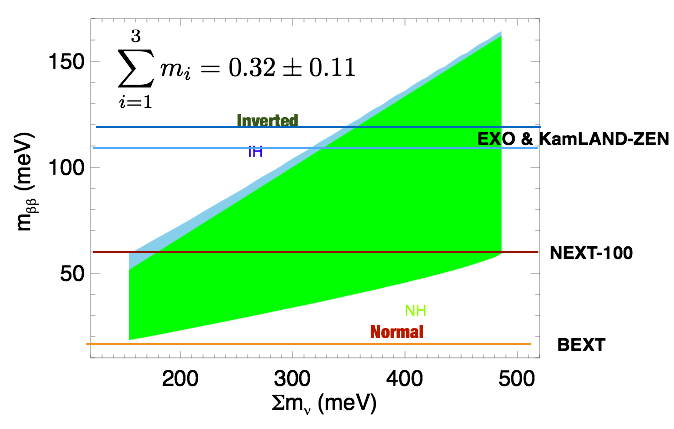
\includegraphics[width=0.70\textwidth]{img/SensiCRR.png}
\caption{\small The allowed \mbb\ region (68\% CL for two degrees of freedom), as a function of the sum of the neutrino masses, assuming that 
$\sum m_i = 0.32\pm 0.11$~eV. The blue lines mark the sensitivity of EXO and KamLAND-ZEN, the xenon-based detectors currently leading the field. The red line shows the sensitivity of NEXT after 3 years operation, which gives the experiment a sizable chance of making a discovery.} 
\label{fig.mbb}
\end{figure}
%%%%%%

 Several analyses from recent cosmological results suggest that the sum of the masses of the three neutrinos could be $\sim$ 0.3 eV\footcite{PhysRevLett.112.051303}. G\'omez-Cadenas and collaborators have demonstrated that, in this case, if the neutrino is a Majorana particle, then, $\mbb \sim [20-150]$~ meV \footcite{GomezCadenas:2013ue}, as shown in Figure \ref{fig.mbb}. In this scenario, the sensitivity of GERDA is outside the ``cosmologically relevant region'' (CRR), while both EXO-200 and KamLAND-Zen would have already explored a significant fraction of CRR {\em for the most optimistic NME set} (while they would be outside CRR for the most pessimistic). 
 
% Clearly, the experimental effort to determine if the neutrino is a Majorana particle, far from being completed is, rather, in its infancy. To establish unambiguously that the neutrino is (or not) a Majorana particle, even in this favourable scenario in which the sum of the neutrino masses is relatively high, experiments must be sensitive to $\mbb \sim 20$~meV, {\em even for the most pessimistic NME} set. On the other hand, a xenon experiment probing a $\Tonu >2.6 \times 10^{25}$~yr, has chances of making a discovery.
% 
 
%%%%%%%%%%%%%%%%%%%%%%%%%%%%%%%%%%%%%%%%%%%%%%%%%%%%%%%%%%%%
\paragraph{The NEXT experiment and its innovative concepts.}
\begin{figure}
\centering
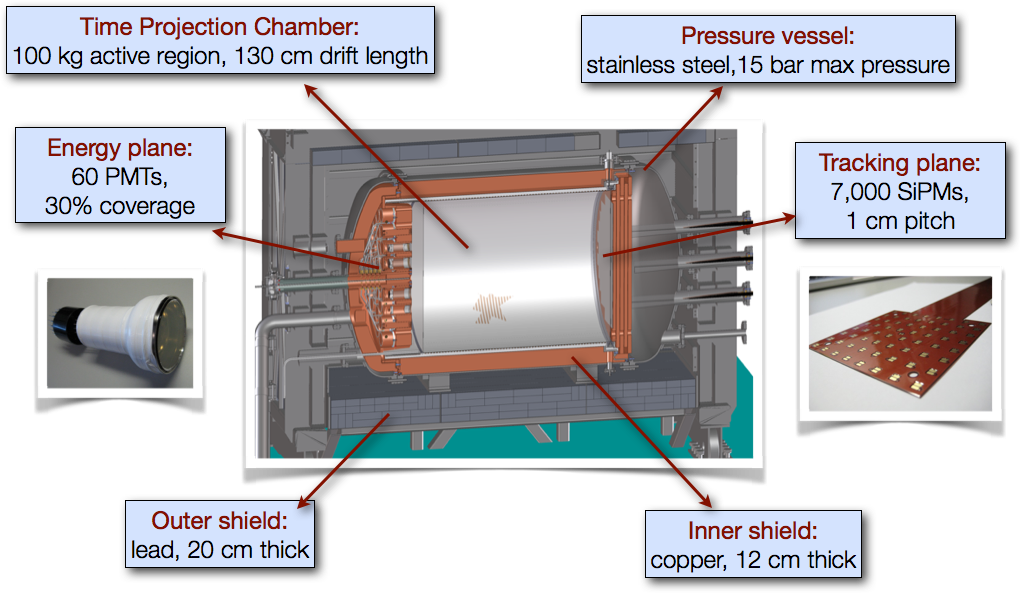
\includegraphics[width=0.9\textwidth]{img/NEXT.png}
\caption{\small A drawing of the NEXT-100 detector showing its main parts. The pressure vessel (PV) is made of a radio pure steel-titanium alloy. The PV dimensions are 130~cm inner diameter, 222~cm length, 1~cm thick walls, fot a total mass of 1\,200 kg. The inner copper shield (ICS) is made of ultra-pure copper bars and is 12~cm thick, with a total mass of 9\,000 kg. The time projection chamber includes the field cage, cathode, EL grids and HV penetrators.
The light tube is made of thin teflon sheets coated with TPB (a wavelength shifter). 
The energy plane is made of 60 PMTs housed in copper enclosures (cans).
The tracking plane is made of MPPCs arranged into dice boards (DB). 
} \label{fig.NEXT100}
\end{figure}

The \emph{Neutrino Experiment with a Xenon TPC} (NEXT)\footcite{next} will search for \bbonu\ in \XE\ using  high-pressure xenon gas  time projection chambers (\HPXE). The advantages of the technology are: 
a) {\bf excellent energy resolution}, with an intrinsic limit of about 0.3\% FWHM at \Qbb, close to that of \GE\ detectors; b)
{\bf tracking capabilities} that provide a powerful topological signature to discriminate between signal (two electron tracks with a common vertex) and background (mostly, single electrons); c)
{\bf a fully active and homogeneous detector}, with no dead regions; d) {\bf scalability} of the technique to large masses; e) the possibility of exciting the barium ion produced in the xenon decay from the fundamental state \TwoS\ to the state \TwoP, using a ``blue'' laser (493.54 nm), and observing the ``red light'' emitted in the transition from \TwoP\ to \TwoD, thus ``tagging'' the presence of a barium atom in the xenon gas, which cannot be produced by any known background. 

The design of the NEXT-100 detector (Figure \ref{fig.NEXT100}) is optimised for energy resolution by using proportional electroluminescent (EL) amplification of the ionisation signal. The detection process involves the use of the prompt scintillation light from the gas as start-of-event time, and the drift of the ionisation charge to the anode by means of an electric field ($\sim0.3$ kV/cm at 15 bar) where secondary EL scintillation is produced in the region defined by two highly transparent meshes, between which there is a field of $\sim20$ kV/cm at 15 bar. The detection of EL light provides an energy measurement using photomultipliers (PMTs) located behind the cathode (the \emph{energy plane}) as well as tracking through its detection a few mm away from production at the anode, via a dense array of silicon photomultipliers (the \emph{tracking plane}).

\paragraph{\label{sec.new}The NEW detector.}

%%%%%%%%%%
\begin{figure}
\centering
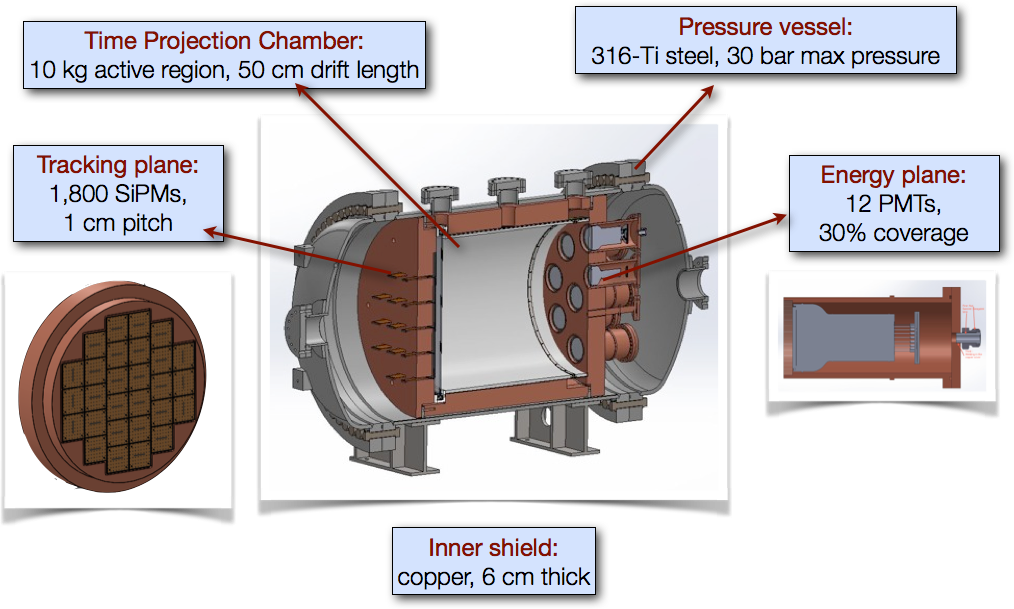
\includegraphics[height=9cm]{img/NEW.png}
\caption{\small The NEW apparatus.} \label{fig:NEW}
\end{figure} 

The NEW (NEXT-WHITE) apparatus\footnote{The name honours the memory of the late Professor James White, one of the key scientists of the NEXT Collaboration.}, shown in Figure \ref{fig:NEW}, is the first phase of the NEXT detector to operate underground. NEW 
%has a triple goal:
%
%\begin{enumerate}
%\item {\bf Technology}: it will validate the technological solutions adopted by NEXT-100.
%\item {\bf Radiopurity}: it will allow the NEXT collaboration an extra step in the implementation of a radiopure detector.
%\item {\bf Physics}: it will demonstrate with measurements of the \BI\ and \TL\ lines, as well as with the measurement of the \bbtnu\ spectrum, the physics capabilities of NEXT-100.
%\end{enumerate}
%
is a scale 1:2 in size (1:8 in mass) of NEXT-100. The energy plane contains 12 PMTs (20 \% of the 60 PMTs deployed in NEXT-100). The tracking plane technology consists of 30 Kapton Dice Boards (KDB) deploying 1800 SiPMs (also 20\% of the sensors). The field cage has a diameter of 50~cm and a length of 60~cm (the dimensions of the NEXT-100 field cage are roughly 1~m long and 1.2~m diameter). 

NEW is a necessary step\footnote{As formally stated by the scientific committee of the LSC, who recommended its construction in 2013.} towards the construction of NEXT-100. It will validate the technological solutions adopted by the collaboration and, as discussed below, it is essential in the definition of the project methodology. Furthermore, The NEXT background model is currently based on a sophisticated Monte Carlo simulation of all expected background sources in each part of the detector. NEW will allow the validation of the background model with actual data. 
%Last but not least, NEW operation will demonstrate with measurements of the \BI\ and \TL\ lines, as well as with the measurement of the \bbtnu\ spectrum, the physics capabilities of NEXT-100.

%Furthermore, the calibration of NEW with 
%sources of higher energy, will allow a precise study of the evolution of the resolution with the energy. 
%In particular it will be plausible to measure the resolution near \Qbb\ using a Thorium source, which provides 2.6 MeV gammas. Last, but not least, we intend to 
%reconstruct the spectrum of \bbtnu. Those events are topologically identical to signal events (\bbonu) and can be used to demonstrate with data the power of the topological signature. 
%
\paragraph{Discovery potential of NEXT-100.}

The excellent resolution of NEXT (0.5 \% FWHM), and the combination of a low radioactive budget with a topological signature (which yields an expected background rate of $5 \times 10^{-4} \ckky$), will allow the NEXT-100 detector to reach a sensitivity to the \bbonu\ period of $\Tonu > 7 \times 10^{25}$~yr for a exposure of 300 kg$\cdot$yr. This translates into a \mbb\ sensitivity range as low as $[67-187]$~meV, depending on the NME. Therefore NEXT-100 will have a substantial chance of making a discovery if the NME is sufficiently high (see Fig.~\ref{fig.mbb}). 

\paragraph{Towards a ton-scale high-pressure xenon TPC (BEXT).}

%%%%%%
\begin{figure}
\centering
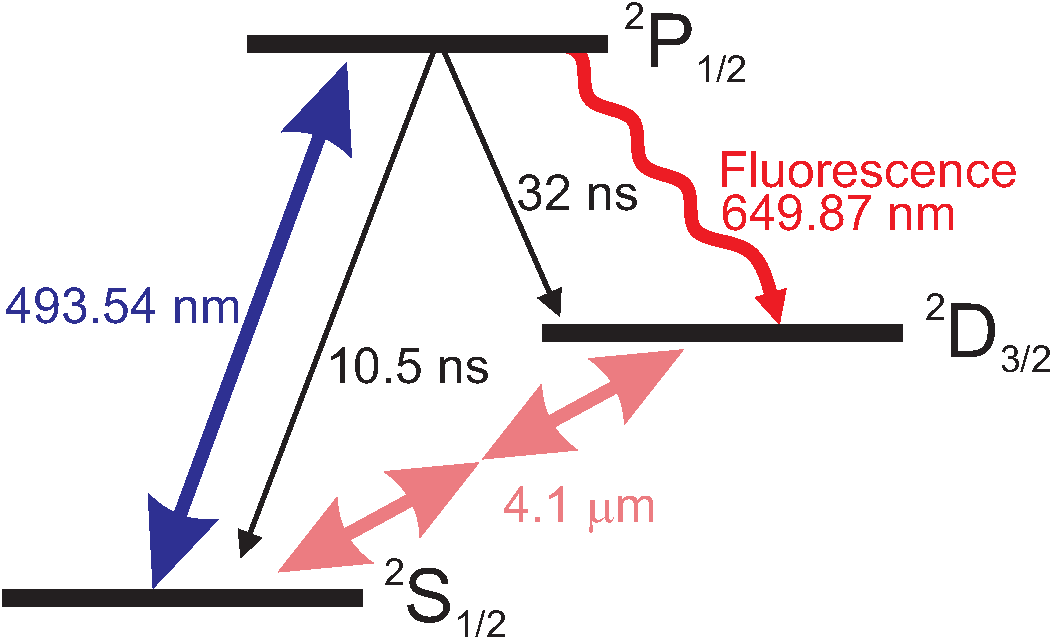
\includegraphics[width=0.50\textwidth]{img/levelscheme2.pdf}
\caption{\small The \BATA\ concept.} \label{fig.BATA}
\end{figure}
%%%%%%

If no discovery is made by the current generation of experiments, the full exploration of the CRR region (corresponding to the inverted hierarchy of neutrino masses, and \mbb\ values as low as 15~meV) requires detectors of larger mass (at least 1 ton), good resolution and extremely low specific background. The \HPXE\ technology has the potential to provide the most sensitive detector at this scale, by scaling the detector to a mass in the range of one ton and adding additional handles to further suppress the background. 

One of the most promising possibilities is to develop the technology to unambiguously tag the barium ion produced in the xenon decay, $Xe \rightarrow Ba^{++} + 2 e^-$. The conceptual idea to tag $Ba^{+}$ is illustrated in Figure \ref{fig.BATA}. A ``blue'' laser of wavelength 493.54 nm excites (``pumps'') the S state, inducing $S \rightarrow P$~transitions, with a lifetime of $\sim$ 10 ns. About 30 \% of the times the \TwoP\ states decay to the state \TwoD, emitting ``red'' (649.76 nm) fluorescence in a characteristic time of 30 ns. The state \TwoD\ is metastable, but a second laser of suitable wavelength (4.1 $\mu$m) can be used to induce the transition to the ground state (this is known as ``deshelving'').  The whole cycle takes less than 50 ns, and therefore several millions of red fluorescence photons can be emitted by a single ion. 

The practical application of this conceptual idea is by no means easy, and in fact, it has been shown to be extremely difficult in liquid xenon by the work of the EXO collaboration\footcite{Dolinski:2012dta}. However, it may be feasible in a \HPXE\ detector, where a number of fortunate conditions may occur. These conditions are: a) charge reduction of the emitted barium ion, from $Ba^{++}$~to $Ba^{+}$, which can be induced by collisions with xenon atoms, or by the addition of a suitable quencher; b) ``trapping'' of the barium ion ``in situ'' by the surrounding Xe atoms, which result in a very low drift velocity for the ion; c) location of the ion, via the reconstruction of the event topology. 

All the above needs to be demonstrated with a systematic R\&D program, which must also address additional experimental issues such as pressure broadening of the laser, filtering of Rayleigh scattering, and others. Most importantly, such an experimental program must be carried out by an interdisciplinary group, combining the experience in laser spectroscopy and atomic physics, with the experience in \HPXE\ instrumentation.

The on-going collaboration between IFIC (and other groups of NEXT) and CLPU\footcite{clpu}, a national facility dedicated to ultra-intense lasers, has made possible to create precisely the interdisciplinary team needed for a successful R\&D program, which can culminate in a ``Barium-tagging Experiment with a Xenon TPC'' (BEXT). 
A future detector of 1 ton mass, with a resolution of 0.5 \% FWHM and a background rate in the range of $10^{-6} \ckky$~(thanks to the implementation of barium-tagging) would be able to fully cover the CRR (and inverted hierarchy) region in less than 5 years, assuming a favourable scenario for the NME. Even the most pessimistic NME scenario could be fully explored, athough with a longer run, since the sensitivity to the \bbonu\ period increases linearly with exposure for a virtually background free experiment as in this case. 

Clearly the construction of a ton-scale \HPXE\ detector implementing the full \BATA\ technology is a very challenging enterprise. On the other hand, we believe that the incremental approach devised by the NEXT collaboration will work also in this case. The construction of the NEW detector is progressing without significant problems thanks to the expertise and know-how gained during the DEMO phase, and we expect that NEXT-100 will fully benefit from the experience gained with NEW. Similarly, the \BATA\ technology could be ready in a period of 4 years by approaching the problem step by step. This R\&D task can be carried out in parallel with the construction and commissioning of NEXT.


%Si el proyecto es continuación de otro previamente financiado, individual o coordinado, deben indicarse con claridad los objetivos y los resultados ya alcanzados de manera que sea posible evaluar el avance real que se propone en el nuevo proyecto. Si el proyecto aborda un tema nuevo, deben indicarse los antecedentes y contribuciones previas de los equipos de investigación que justifiquen su capacidad para llevarlo a cabo.
%

This research project is the continuation of the CONSOLIDER-INGENIO project CUP (2010-2014), and the SEIDI project FIS2012-37947-C04 (2012-2014). 

The initial phase of the project (called the DEMO phase), included a learning period (2010-2011), needed to acquire the very innovative technology the detector is based on, and to equip state-of-the-art laboratories at IFIC and other participating institutions. 
During 2011 and 2012, the collaboration selected the technology to be implemented and a Technical Design Report\footcite{Alvarez:2012haa} was published in 2012. This phase of the project culminated  with the construction, commissioning and operation of the NEXT-DEMO prototype located at IFIC, and the NEXT-DBDM prototype operating at LBNL. Between 2012 and 2014, the results of the prototypes were analysed and published, showing the excellent performance (energy resolution, electron reconstruction) of the apparatus, as well as the robustness of the EL technology\footcite{Alvarez:2012hh, Alvarez:2012nd, Alvarez:2012hu,Alvarez:2013gxa,Lorca:2014sra}. 

\subsubsection*{NEXT prototypes}

\begin{figure}
\centering
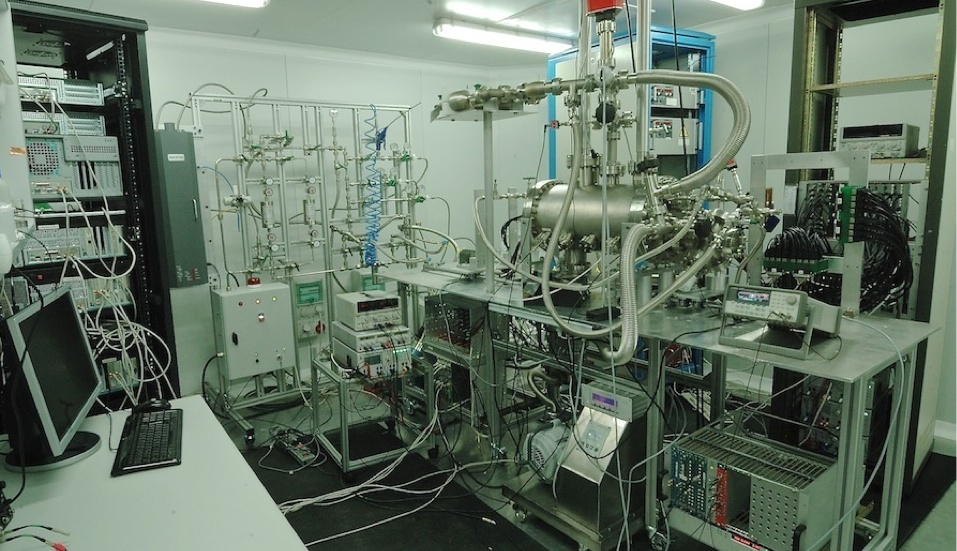
\includegraphics[width=0.7\textwidth]{img/DemoSetup.jpg}
\caption{\small The NEXT-DEMO prototype setup at IFIC.} \label{fig.DEMO}
\end{figure}
%%%%%%%%%%

NEXT-DEMO, shown in figure \ref{fig.DEMO}, is as a large-scale prototype of NEXT-100. The pressure vessel has a length of 60 cm and a diameter of 30 cm. The vessel can withstand a pressure of up to 15 bar and hosts typically 1-2 kg of xenon. NEXT-DEMO is  equipped with an energy plane made of 19 Hamamatsu R7378A PMTs and a tracking plane made of 256 Hamamatsu SiPMs. 

The detector has been operating successfully for more than two years and has demonstrated: (a) very good operational stability, with no leaks and very few sparks; (b) good energy resolution ; (c) track reconstruction with PMTs and with SiPMs coated with TPB; (d) excellent electron drift lifetime, of the order of 20 ms.Its construction, commissioning and operation has been instrumental in the development of the required knowledge to design and build the NEXT detector.

The NEXT-DBDM prototype is a smaller chamber, with only 8 cm drift, but an aspect ratio (ratio diameter to length) similar to that of NEXT-100. The device has been used to perform detailed energy resolution studies. NEXT-DBDM achieves a resolution of 1\% FWHM at 660 keV and 15 bar, which extrapolates to 0.5\% at \Qbb.

\subsubsection*{Topological signature}

%%%%%
\begin{figure}
\centering
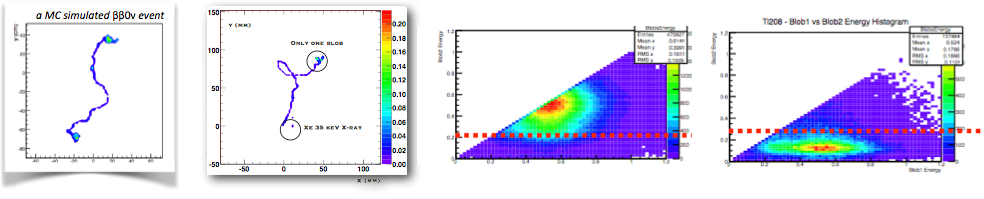
\includegraphics[width=0.9\textwidth]{img/Topo2.png}
\caption{\small NEXT has a topological signature, not available in most \bbonu\ detectors. The panel shows the reconstruction of a Monte Carlo signal (topleft) and background (bottomleft) event. The signal has two electrons (two blobs). The background has only one electron (one blob) and the associated emission of a 35 keV X-ray. The color codes energy deposition in the TPC. An scatter plot of the energy of the two blobs shows a clear separation between signal and background regions.}\label{fig.ETRK2}
\end{figure}
%%%%%

%%%%%%
%\begin{figure}
%\centering
%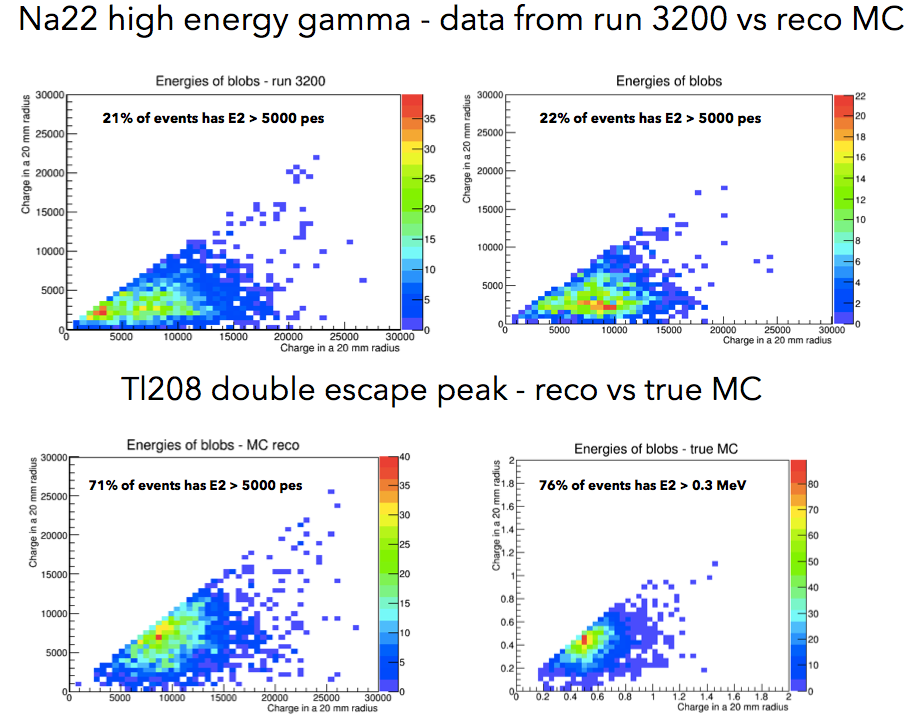
\includegraphics[width=0.9\textwidth]{img/ElectronsDataMC.png}
%\caption{\small A comparison between data (left) and Monte Carlo (right) for electrons of different energies recorded in the DEMO chambers, showing the very good agreement between both data sets and therefore the robustness of the topological signal, unique of the NEXT experiment.}\label{fig.ETRK3}
%\end{figure}
%

Double beta decay events leave a distinctive topological signature in HPXe: a continuous track with larger energy depositions (\emph{blobs}) at both ends due to the Bragg-like peaks in the d$E$/d$x$ of the stopping electrons (figure \ref{fig.ETRK2}, topleft). In contrast, background electrons are produced by Compton or photoelectric interactions, and are characterised by a single blob and, often, by a satellite cluster corresponding to the emission of $\sim30$-keV fluorescence x-rays by xenon (figure \ref{fig.ETRK2}, bottomleft).
Reconstruction of this topology using the tracking plane provides a powerful means of background rejection, as can be observed in the figure. 
%In our TDR we chose a conservative cut to separate double--blob from single--blob events which provided a suppression factor of 20 for the background while keeping 80\% of the signal.  DEMO has reconstructed single electrons from \NA\ and \CS\ sources, as well as double electrons from the double escape peak of \TL\, demonstrating the robustness of the topological signal. 

%
%Figure \ref{fig.ETRK3} shows a comparison between data and Monte Carlo for electrons interacting in the DEMO detector. Two radioactive sources were used: Na-22, producing single electrons of 511 keV, and Tl-208, whose double escape peak produced {\em double electrons}, at the energy of 1.6 MeV. Both data sets allow us to ``mimic'' signal and background and thus have a robust assessment of the performance of the topological signal comparing the Monte Carlo simulation and the actual results obtained with DEMO. The agreement between both data sets is very good, revealing the robustness of the topological signal. 

\subsubsection*{Energy resolution}

%%%%%
\begin{figure}
\centering
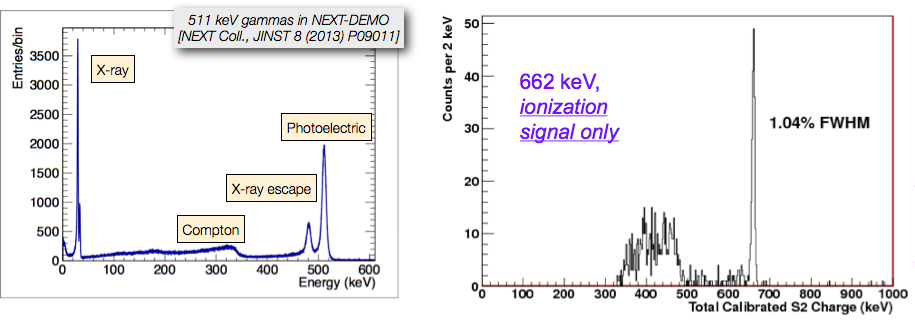
\includegraphics[width=0.8\textwidth]{img/EResolution.png}
\caption{\small Left: the full energy spectrum measured for electrons of 511 keV in the DEMO detector. Right the spectrum near the photoelectric peak for 662 keV electrons in NEXT-DBDM. The resolution at 662 keV is 1\% FWHM (0.5\% FWHM at \Qbb). The resolution extrapolated from 511 keV is 0.7\%.}\label{fig.ERES}. 
\end{figure}
%%%%

Figure \ref{fig.ERES} shows the resolution obtained with the NEXT-DBDM apparatus. A resolution of 1\% FWHM with 
662 keV photons, has been measured, which extrapolates to 0.5\% FWHM at \Qbb. This result is not far from the expected limit obtained adding in quadrature the different factors that contribute to the resolution (Fano factor, photoelectron statistics and electronic noise). The resolution measured in NEXT-DEMO extrapolates to 0.7\% FWHM. The difference between both prototypes is due to better photoelectron statistics and aspect ratio in DBDM. The results, are, in any case, better than the target of 1\% FWHM described in the TDR.

The status of the NEXT experiment and the results achieved by the prototypes have been described in a recent
paper \footcite{Gomez-Cadenas:2013lta}.



\subsubsection*{Objetivos generales y adecuación al Programa Estatal de I+D+i orientada a los Retos de la Sociedad / General objectives and match to the National Programme for research aimed at the Challenges of Society}

%\subsection*{Objectives and methodology}

%2. La hipótesis de partida y los objetivos generales perseguidos con el proyecto coordinado en su conjunto, así como la adecuación del proyecto a la Estrategia Española de Ciencia y Tecnología y de Innovación y, en su caso, a Horizonte 2020 o a cualquier otra estrategia nacional  o internacional de 

The overall objectives of this research proposal are:

\begin{enumerate}
\item Construction, commissioning and operation of the NEW and NEXT-100 detectors, during a period of 4 years, from 2015 to 2019.
\item Demonstrate the feasibility of barium tagging in an HPXe, performing a systematic set of small, focused, prove-of-concept experiments. As a part of this objective, an infrared laser using innovative technology will be developed. 
\end{enumerate}
  
The COORD subproject leads the construction of the NEW and NEXT-100 detectors, while the ENG subproject leads the deployment of the electronics, DAQ and slow controls. The CALREC subproject leads the calibration of the detector. The R\&D for barium tagging is lead by the BATA subproject (CLPU), with the participation of all the groups.   

The specific objectives of all the sub projects are integrated in the NEXT Project Management Plan. 
The PMP coordinates the construction of the NEW and NEXT-100 detectors. It is under the direct supervision of the Spokesperson (SP) and the Project Manager (PM). The PM of NEXT is Dr. I. Liubarsky, part of the IFIC group. 

The PMP defines a set of Working Packages (WP) and follows the progress of each one, monitors deliverables and dead lines and keeps track of invested resources including personnel. It also identifies potential show-stoppers and synergies (and possible conflicts) between the different projects and optimises the sharing of resources. 

%Figure \ref{fig.Gantt} shows an example of the Gantt chart for the whole NEW project, up to installaton at the LSC. 

%The objectives defined for the different sub projects match the various WP in the PMP, as can be seen in Figure \ref{Fig:PMP}. 

The methodology of each WP includes: a) the definition of the associated tasks; b) the identification of the resources needed; c) the temporal organisation of the tasks; d) the definition of milestones and the deliverables associated to them; e) the relations with other WP. Each WP has a leader, which reports directly to the PM. The progress of each WP is reviewed on a weekly basis. Milestones and potential showstoppers are discussed, and the tracking charts updated if needed. The PMP is reviewed every six months by the LSC scientific committee.  

The objectives presented in this project are very well aligned to the spanish program for science, as demonstrated by the fact that NEXT has been supported by the CONSOLIDER-INGENIO project CUP. The support of the AdG/ERC makes it clear that the projects suits perfectly well the goals of H2020. NEXT is a CERN recognised experiment and has been listed by NSA\footcite{NLDBD} as one of the key \bbonu\ experiments in the field, and the one with best future prospects.





%Si la memoria se presenta a la convocatoria de RETOS INVESTIGACIÓN, deberá identificarse el reto cuyo estudio se pretende abordar y la relevancia social o económica prevista.
%
This research project is presented within the program of ``Challenges of society'', specifically, challenge number 6: {\bf Change and social innovation.}

We argue that this project represents a major innovation in the way that particle physics is conducted in Spain, and thus marks a path to a more productive approach to research.

Particle physics is a clear example of the so-called ``big-science''. The discovery of the Higgs boson is a quintessential example of such big science. It has required the construction and operation of the LHC, one the most impressive scientific machines ever built by humankind. The gargantuan scale of the effort could only be met by a collective effort centralised at CERN, the largest particle physics laboratory in the World.  

Big science involves big budgets, often invested in purchasing equipment to be installed at CERN and in paying scientific staff whose activity also develops at CERN. Such large budgets are often justified in terms of industrial and scientific returns. While those returns certainly exist, {\bf they tend to be larger for countries who are already well developed scientifically}. Specifically, the positions of leadership in the large CERN experiments, and in the CERN scientific and technical divisions, are dominated by countries like Germany, Switzerland, U.K., France and Italy. 

Remarkably, the countries leading the big science at CERN and other laboratories have also developed ``national science'' physics programs. A case of great interest is Italy, a country not very different from Spain, in terms of GDP and social habits. However, the international impact and the returns of physics in Italy is much larger than in Spain. For example, the number of spanish staff members at CERN is 115, to be compared with 275 corresponding to Italy (which has the second largest staff population, after France, who co-hosts the lab). Adding fellows and associates (that is, temporary CERN contracts, often given to scientists), the figures for Spain are 363, to be compared with 1726 for Italy\footnote{\href{http://council.web.cern.ch/council/en/Governance/TREF-PersonnelStatistics2012.pdf}{http://council.web.cern.ch/council/en/Governance/TREF-PersonnelStatistics2012.pdf}}. Several Italians have served as CERN general directors, and have led or are leading the LHC experiments. The next CERN general director (and perhaps the first woman to occupy such position in the history of the lab) may be the ex-spokesperson of ATLAS, the italian physicist Fabiola Gianotti. Moreover, Italy has four Nobel prizes in physics (Marconi, 1909, Fermi, 1938, Segrè 1959, Rubbia 1984), while Spain has none. 

Remarkably Italy also boasts the best underground laboratory of Europe, and one of the best of the world, the LNGS. The lab hosts 20 experiments including three searching for \bbonu\ processes (GERDA, CUORE and COBRA) and two experiments searching for Dark Matter (WARP and XENON). 

Through these experiments, the italian physics{\bf attracts external talent} (some of the best physicists from Europe and USA participate in experiments at LNGS) {\bf and external funding}, complementing the big science at CERN with physics of a smaller scale concerning human resources and budgets. However, such ``local'' physics results in discoveries of great scientific impact (such as the discovery of neutrino oscillations, which has been the result of a world-wide effort involving underground laboratories in Italy, USA, Canada, Russia and Japan). It also allows the training of students and post-docs in experiments where young physicists can make a major impact at all levels, ranging from the construction of the detector to the analysis of the data. Last, but not least, such local science has an important impact in the italian industry and in the appreciation of science by the public in general. 

{\bf We argue that, in order to balance and optimise the current big-science effort in Spain, it is necessary to develop the physics at the LSC, in analogy to the italian case.} NEXT is the flagship experiment of our national laboratory, and has achieved intentional recognition, as demonstrated by the fact that is a recognised CERN experiment and has obtained an AdG/ERC, {\bf the first grant of this type in the field of particle physics}. 

We, therefore, consider that the NEXT project is a clear example of social innovation, as it has the potential of implementing profound changes in spanish science. As described in this project, NEXT, through its various stages, can hit a major discovery. It will bring international credit and visibility to our science and to the LSC. And it has an important impact both in local industry (through contracts to many national firms, and development of high technology) and in the public perception of science. 

Furthermore, the on-going collaboration with the CLPU further reinforces the above arguments, since the effort involves now a second national scientific installation. In addition, the \BATA\ program implies a major example of inter disciplinarity, and can result in a number of important technological returns (development of infra-red laser technology, which has a myriad scientific and technological applications).

Finally it is important to remark that, while the usual operation of big-science in Spain implies to finance the participation of our groups (including the annual CERN quota, the common-fund of the experiments and the contributions to construction and operation of the CERN experiments), the national science that NEXT represents obtains external funding through ERC projects (including the AdG and several H2020 actions currently in progress involving LSC), as well as the contributions of the international collaboration to detector construction and operation (in particular, in the case of NEXT through the USA groups led by Prof. Dave Nygren, the inventor of the technology in which NEXT is based). NEXT also attracts external talent to our country (as the intense collaboration with top USA universities demonstrates). The NEXT group is very international, and several of our post-docs are or have been financed by EC grants (such as the Marie Curie). 

Last but not least, the NEXT experiment, and in particular the collaboration with the CLPU, involves the extensive development of photonics listed as one of the  ``Facilitating Essential Technologies''.

\subsubsection*{Objetivos específicos / Specific objectives}
%

% Los objetivos específicos de cada uno de los subproyectos participantes, enumerándolos brevemente, con claridad, precisión y de manera realista (acorde con la duración prevista del proyecto).
%
% En los subproyectos con dos investigadores principales, deberá indicarse expresamente de qué objetivos específicos se hará responsable cada uno de ellos.
%

\subsubsection*{Objectives of the COORD subproject}

\begin{figure}
\centering
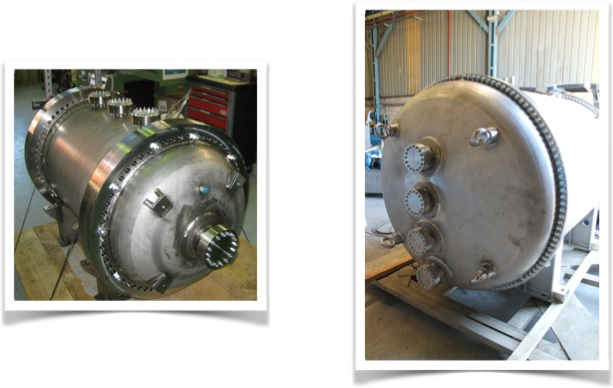
\includegraphics[height=8cm]{img/PV.jpg}
\caption{The pressure vessel of NEW (left) and NEXT-100 (right).} \label{fig:PV}
\end{figure}

%%%%%
\begin{figure}[t!b!]
\begin{center}
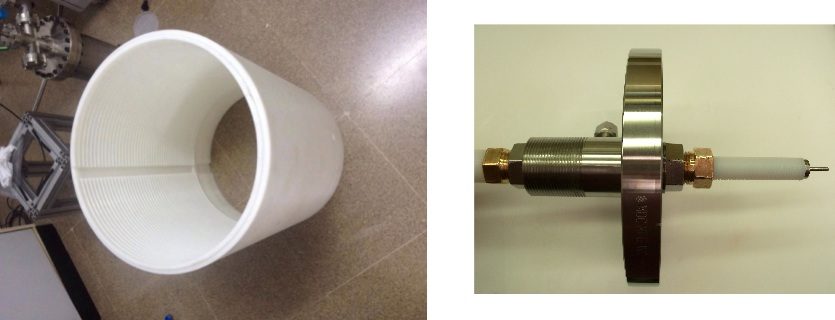
\includegraphics[width=.9\textwidth]{img/FC3.jpg}
\end{center}
\caption{Left: The NEW field cage body made of HDPE, fabricated in Spain; right: The anode HVFT manufactured in Texas.
} \label{fig:FC}
\end{figure}

%%%%%
\begin{figure}[t!b!]
\begin{center}
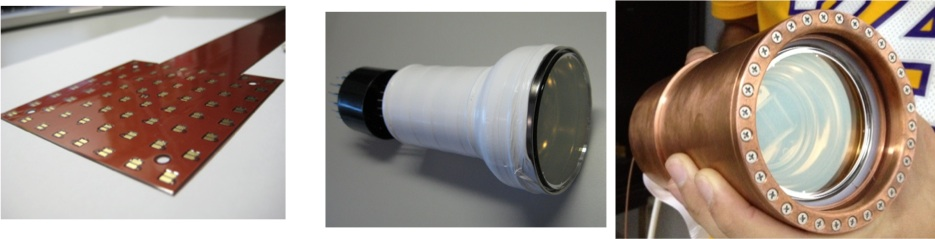
\includegraphics[width=.9\textwidth]{img/KDBandPMT.jpg}
\end{center}
\caption{Top left: the flexible Kapton Dice Board (KDB) circuit developed by NEXT for the tracking plane; mid: the R11410-10 PMT from Hamamatsu; bottom right: a PMT can prototype.} \label{fig:sensors}
\end{figure}

The specific objectives of the COORD subproject are:

\begin{enumerate}
\item {\bf Construction of NEW}, foreseen to be completed in Q2'15, and involving:
\begin{enumerate}
\item {\em Construction of the NEW and NEXT-100 pressure vessels}.
The NEW and NEXT-100 pressure vessels, shown in Figure \ref{fig:PV} were designed to withstand pressures in excess of 20 bar, and to operate with negligible losses at 15 bar. They are built using a 316Ti alloy of low activity. 
The design was a collaboration between IFIC and LBNL groups. They have been manufactured by several Spanish companies (TRINOS, MOVESA and ACYM). Currently (Q4'14) the NEW pressure vessel (NPV) is being fitted with a copper shield (called the Inner Copper Shield, ICS) that attenuates residual ambient radiation. NPV will be shipped tested for functionality at IFIC in Q1'15, then shipped to LSC and commissioned during Q2'15. 

\item {\em Construction of the NEW field cage (NFC)}
The NEW field cage produces an uniform electric ($\sim$ 300 V/cm) field inside the  detector that drifts the ionisation electrons to the anode, where they are further accelerated in the electric field produced between a pair of transparent grids, called the electroluminescent (EL) grids. 

The main body of the field cage is a high density polyethylene (HDPE) cylindrical shell with a 2.5\,cm wall thickness (Figure \ref{fig:FC}, left).  The drift region consists of radiopure  copper strips connected with low radioactivity resistors.  The light tube consists of thin sheets of teflon, coated with tetraphenyl butadiene (TPB). The role of the TPB is to shift the UV light produced in xenon to the blue region (PMT and SiPMs operate best in this region, around 450 nm).  A high-voltage feedthrough (HVFT) in the cathode and another one in the anode, allow the definition of the voltages (Figure \ref{fig:FC}, right). The cathode HVFT is designed to withstand up to 100 kV, and the HVFT of the anode to withstand up to 40 kV. The design of the HVFT, identical for NEW and NEXT-100 improve those that were built for DEMO by the Texas A\&M group. The field cage and grids of NEW and NEXT-100 are also identical, to a scale 1:2. The grids use a stainless steel mesh with pitch 0.5 mm and wire diameter 30 microns, which results in an open area of 90\%. 

The construction of NFC is currently under way (Q4' 2014). The HDPE body has been fabricated by the spanish company AIMPLAS. The HVFT and the grids have been manufactured at Texas. The  NFC will be tested at IFIC before shipping and installation in the LSC in Q1'15. The field cage will be commissioned in Q2'15. System commission, together with the rest of the systems will occur during Q3'15 and Q4'15.

\item {\em Construction of the NEW energy plane (NEP)}
In NEW the energy measurement will be provided by the detection of EL light via PMTs, which will also record the scintillation light needed for $t_0$. Those PMTs will be located behind a transparent cathode.

A total of 12 low-background, high-QE PMTs, model R11410-10 from Hamamatsu (Figure  \ref{fig:sensors}, mid panel) covering 32.5\% of the cathode will be deployed. The R11410-10 are large tubes, with a 3'' photocathode and low levels of  activity of the order of 1 mBq per unit in the Uranium and Thorium series. The PMTs are sealed into individual pressure resistant, vacuum tight copper enclosures (called PMT cans) coupled to 
sapphire windows, coated with ITO (for electrical conductivity) and TPB (Figure  \ref{fig:sensors}, right panel).

The NEW energy plane (NEP)
is currently (Q4'15) under construction at IFIC. The ``PMT can'' design have been validated and production of the parts has started. The NEP will ship to LSC during Q1'15. It will be commissioned in Q2'15. System commission, together with the rest of the systems will occur during Q3'15 and Q4'15.

\item  {\em  Construction of the NEW tracking plane (NTP)}:
In NEW the tracking function is provided by a plane of multi-pixel photon counters (SiPMs) operating as a light-pixels and located behind the transparent EL grids. They are mounted in flexible radiopure Kapton Dice Boards (KDB). Each KDB hosts 64 SiPMs (Figure  \ref{fig:sensors}, left panel) .The NTP will deploy 28 such KDBs. 

The NTP is currently under construction at IFIC (Q4'14). The KDB production has been validated and prototypes have demonstrated excellent performance. The NEP will ship to LSC during Q1'15. It will be commissioned in Q2'15. System commission, together with the rest of the systems will occur during Q3'15 and Q4'15. 

\end{enumerate}
 
\item {\bf Commissioning of NEW and evaluation of performance}. The NEW detector will be brought online in Q2'15, and extensive system testing will be performed to certify safe and stable operation (no leaks, no sparks), as well as testing and integration of all the subsystems. We expect to complete commissioning in Q3'15.
During Q4'15, we will evaluate the performance of the detector. Such evaluation will allow us to correct for design problems (if they arise) or to introduce improvements in the engineering if needed. We will also assess the overall radioactive budget of the detector, to ensure the absence of ``hot spots'' (excess of radioactivity introduced accidentally in the detector). 

\item {\bf NEW physics run}. During 2016, we will operate continuously the NEW detector at the LSC. The physics runs of NEW has several goals: a) measurement, using radioactive sources, of the energy resolution as a function of the energy, and in particular at \Qbb (CALREC subproject) ; b) measurement, using radioactive sources, of single (``background'') electrons, as well as ``double electrons'' (produced by the double escape peak of Tl-208, and used to characterise the signal) (COORD and CALREC); c) measurement of the standard mode \bbtnu; and d) a full measurement of the spectrum, after selection cuts, thus quantifying, from the data themselves, the background model (collaboration wide studies). 
%

\item {\bf Construction of NEXT-100}. The fabrication of NEXT-100 will proceed through 2016, although some parts (such as the pressure vessel) have already been built. 
The construction will take 12 months. This fast schedule is possible thanks to several factors:
\begin{enumerate}
\item {\em Reuse of infrastructures}: the platform, pedestal, lead castle, gas system, clean tent, radon suppression system, online computing, slow controls and calibration hardware and procedures are common to NEW and NEXT-100 and will be extensively tested during NEW operation, thus ready for NEXT-100 phase.
\item {\em Early construction of pressure vessel}: The pressure vessel is a critical system, since it has to operate underground, at high pressure and with negligible losses. Designing, constructing and certifying it takes a long time. Luckily, this fact was understood at an early stage in the development of the project and the NEXT-100 pressure vessel (see Figure \ref{fig:PV}) was constructed during 2014, and has been tested and certified at the same time than the NEW pressure vessel. 
\item {\em Scalability of the field cage}: Some of the most delicate subsystems of the field cage (such as the HVFT) have been designed and tested to be operative in NEXT-100 (for example the HVFT in the cathode holds up to 100 kV voltage, while the nominal operation of NEXT-100 is 50 kV). The NEXT-100 field cage body will be constructed by the same company (AIMPLAS) that has built the NFC body, reusing the tools and procedures that have been put together for the task. This also applies to the construction of the EL grids. 
This makes possible to foresee an early assembly of the NEXT-100 field cage, in Q2'16, allowing for ample time for testing and debugging.

\item {\em Production chains for the energy and tracking planes}. The energy and tracking planes are composed of individual modules (PMT cans in the case of the energy plane, KDBs in the case of the tracking plane), mounted to supporting plates and connected to electronics. The structure of the systems is the same (as seen in Figure \ref{fig:EnergyPlane}). The number of modules (cans and KDBs) is larger in NEXT-100 (by about a factor 5), but, very importantly, the construction procedure is the same. This allow us to set {\em production chains}, PC, of both PMT cans and KDBs. The PCs will be extensively exercised during the construction of NEW, and are expected, therefore, to run smoothly during NEW construction.  

The production chains should be able to produce 20 PMT cans and 30 KDBs a month. We therefore, expect that the modules will be ready in Q1'16. Shipping and cleaning will take the best part of Q2'16. The systems should be assembled at the LSC in Q3'16, allowing for testing and debugging during Q4'16.
\end{enumerate}

\item {\bf Commissioning of NEXT-100}. The commissioning of NEXT-100 will benefit from the experience gained commissioning and operating NEW. We consider feasible to commission the detector during the first 2 quarters of 2017, but our project management plan allows for two extra quarters. The main reason is to guarantee enough time to run with normal xenon before circulating the precious enriched xenon in the gas system and the detector. Notice that the detector can be fully calibrated, and the backgrounds can be characterised with normal xenon.  

\item {\bf Physics run of NEXT-100}. The physics run may start in the third quarter of 2017, but the project plan foresees the first quarter of 2018. The calibration procedures are identical to those developed for NEW. After one year of run, NEXT-100 should reach the sensitivity of the current leading experiments. We currently foresee to run for three years (2018 to 2020), achieving a sensitivity to \mbb\ that makes a discovery possible if NME are sufficiently large and the neutrino is a Majorana particle. 

\end{enumerate}

% Los objetivos específicos de cada uno de los subproyectos participantes, enumerándolos brevemente, con claridad, precisión y de manera realista (acorde con la duración prevista del proyecto).
%
% En los subproyectos con dos investigadores principales, deberá indicarse expresamente de qué objetivos específicos se hará responsable cada uno de ellos.
%

\subsubsection*{Objectives of the ENG subproject}

\begin{figure}[h!]
\begin{center}
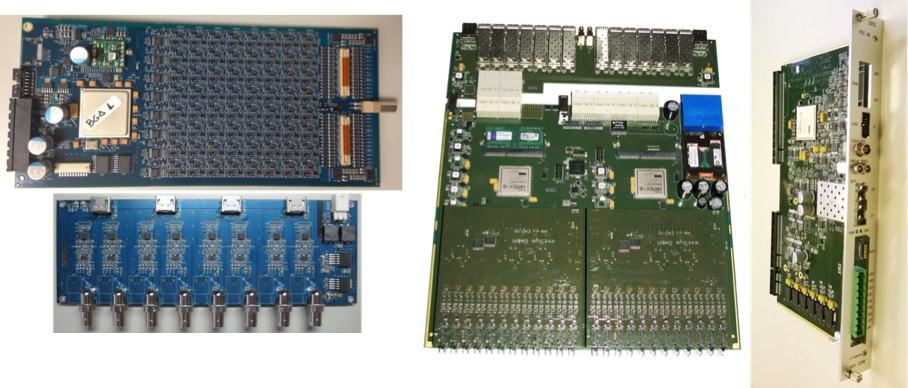
\includegraphics[width=0.9\textwidth]{img/Electronics.jpg}
\end{center}
\caption{\label{Fig:FEE} Left: Front-end boards for SiPM (top) and PMTs (bottom) for NEW and NEXT-100; right: SRS FEC modules in ATCA form factor (left) and “SRS classic” flavour (right) }
\end{figure}

The ENG subproject centralises the front-end electronics, data acquisition (DAQ), online system and slow controls of the NEW and NEXT-100 detectors. It is coordinated by the UPV.
NEXT (via the UPV team) has co-developed a new readout and DAQ concept named SRS \footcite{Toledo2011,SRS2013},for the international RD-51 collaboration at CERN. NEXT front-end modules are connected via copper links to the SRS DAQ interface modules. the CERN standard DATE environment is used as DAQ software. This brings a number of advantages, like counting on a large base of users and developers, reducing production costs and profiting from other group’s developments. SRS has been successfully used in NEXT-DEMO (PMT and SiPM readout, DAQ interface and trigger modules)\footcite{Gil2012,Herrero2012,Esteve2012} and newer versions of these modules are to be used in NEW and NEXT-100\footcite{TWEPP2014}.

The specific objectives of this sub-project are:

\begin{enumerate}

\item {\bf FEE (Front End Electronics)}: Design, fabrication and commissioning of the front-end electronics for the PMTs and the SiPMs for NEW and NEXT-100. The NP leader is the co-PI of the subproject, Prof. Francisco Toledo (UPV).
\begin{enumerate}
\item	{\em Commissioning NEW front-end electronics in 2015}. As an outcome from two previous projects (CUP and FIS2012-37947-C04-04), the front-end electronics for both the PMT plane and the SiPM plane in NEW are available. The former is already being used in NEXT-DEMO while the latter, an evolution from the NEXT-DEMO electronics, exists as prototype boards and will be available in adequate quantities by the end of 2014. Required cabling, power supplies and mechanical structures have already been purchased.
These electronics will be tested at IFIC in Q1’15 and at the LSC in Q2’15. A study on reliability, performance and signal noise will be carried out during the commissioning phase, resulting either on the final validation of the current designs or on a proposal for changes. In this case, the changes will be carried out in Q4’15 and Q1’16.

\item {\em Production, installation and test of NEXT-100 front-end electronics in 2016}. Lessons learnt with NEW commissioning and initial operation will lead to a document on recommendations for installation and operation of electronics in NEXT-100. The specificity of LSC in terms of grounding and power distribution in the experimental area, together from noise in the power lines and generated by neighbouring experiments, will determine the required noise-reduction techniques (mostly ground connections and ad-hoc filtering). After completing the eventual modifications in the front-end modules (Q1'15), production for NEXT-100 in Q2’16, and Q3'16, module test in Q4’16 will complete the 2016 work plan.

\item {\em Commissioning and Operation of NEXT-100 front-end electronics in 2017}. Potential problems found after installation in a detector of the size of NEXT-100 will be addressed. Front-end firmware may require fine adjustments to (1) ease later energy measurement and tracking algorithms and (2) adjust the trigger algorithms as specified for the different physics campaigns. Commissioning is scheduled for Q1-Q2’17. Operations starts on the second half of the year.
\end{enumerate}
 
\item {\bf DAQ}: Design, fabrication and commissioning of the data acquisition modules for NEW and NEXT-100. The NP leader is the second co-PI of the subproject, Prof. Raul Esteve (UPV).

\begin{enumerate}

\item	{\em Commissioning NEW DAQ interface electronics in 2015}. The DAQ interface modules for NEW and NEXT-100 are also available in two flavours: “classic” SRS modules (19” Eurocard form factor, available from CERN Store) and industry-standard ATCA SRS modules. NEW DAQ will use in a first stage modules from both flavours.

These electronics will be tested at IFIC in Q1’15 and at LSC in Q2’15. A study on reliability and performance will be carried out during the commissioning phase, allowing to choose the best solution for NEW and NEXT-100. 
%A third option, a new SRS solution for very-close-to-detector readout codenamed OC-Box, which is to be developed in collaboration with RD51 and intended as an upgrade for NEXT, will be evaluated in 2015 as a future upgrade. It is based on newer FPGA technology and can replace current FEC modules.

\item	{\em Production, installation and test of NEXT-100 DAQ electronics in 2016}. Lessons learnt with NEW commissioning and initial operation will lead to a decision to go for “classic” or ATCA SRS flavor. Purchases for NEXT-100 in Q2’16, module test and firmware upgrade in Q3’16 and installation in Q4’16 will complete the 2016 work plan.

\item	{\em Commissioning and Operation of NEXT-100 DAQ electronics in 2017}. DAQ performance and functionalities will be verified and adjusted to meet final NEXT-100 requirements. DAQ firmware may require some modifications to (1) ease energy measurement and tracking algorithms and (2) adjust the trigger algorithms as specified.

%\item	NEXT-100 operation in 2018. The DAQ requires no maintenance during operation other than module replacement due to damage or malfunctioning. Placed outside the lead castle in 19” racks next to the front-end modules, the DAQ electronics are easily accessible.

\end{enumerate}

\item {\bf Slow control}: Design, fabrication and commissioning of the slow control for NEW and NEXT-100. The project leader is technical engineer Vicente Álvarez, under the supervision of co-IP J. Toledo. The goals are (1) monitor critical detector parameters, mostly temperature and pressure, (2) control power supplies for the sensors, detector grids and electronics and (3) implement an automatic emergency response monitor.
Six subsystems or partitions have been defined: (1) high-voltage sources for PMTs, (2) low-voltage sources for SiPMs and electronics, (3) high-voltage for grids, (4) gas system status -getters, pump and gas recirculation-, (5) a group of temperature and pressure sensors and (6) the main control panel (with cameras and status overview). Partitions are interconnected via Ethernet. Basic functionalities for all subsystems have been implemented in 2014.

%Power supplies for PMTs and SiPMs are directly controlled to Ethernet. Power supplies for the electronics are controller from a PC via USB, being this PC connected to Ethernet. The other subsystems are controlled via a National Instrument’s Compact-RIO chassis with Ethernet link, embedded in a so-called “Slow Control Box”, which includes relays and connections. A LabView software application will be used for the main control panel.

\begin{enumerate}
\item {\em Design, production and commissioning NEW slow-controls in 2015}. The Slow Controls for NEW will be completed in Q4’14, tested and debugged in  Q1’15 and installed in LSC in Q2’15.

%\item {\em Production, installation and commissioning of NEXT-100 slow-controls electronics}. Monitoring the gas subsystem will be an addition to the Slow Controls for NEXT-100 in 2016.
\end{enumerate}

\item {\bf Online}: Design and commissioning of the online system for NEW and NEXT-100. Interfaces with offline, DAQ and Slow Control. The project leader is Dr. Raúl Esteve. The Online System for NEW comprises the following subsystems: (1) Data Storage, (b) Backup Storage, (c) Pre-processing and (d) Online Monitoring. The DAQ System (a PC farm comprising Local and Global Data Concentrators) produces approx. 30 MByte/s in NEW, which are stored into the NEW Data Storage (up to 8 servers with 8 disks each for up to 65 TByte). The Data Storage has power redundancy and multiple network cards per PC for enhanced reliability. Long-term data selected by the Offline System are stored into the Backup Storage (composed of a server PC and a tape server using 1.5 TByte tapes). The Pre-processing comprises two servers which read event data from the Data Storage and apply a format for later offline processing. Finally, a server in the Online Monitoring is used to gather statics, measure performance, find out bottlenecks and check the health of the different subsystems. A 1-Gb Ethernet switch interconnects the PC servers in the Online System, using virtual LANs to separate different data flows.
Backup Storage, Pre-Processing, Data Storage and Online Monitoring have been tested.
%\begin{enumerate}
%\item {\em Commissioning NEW Online system in 2015}. Required hardware elements have either been already purchased of will be purchased before the end of 2014. Prototypes for each sub-system have been already constructed and tested in 2014. The main task in 2015 is to tune the system for NEW operation.
%\item {\em Production, installation and test of NEXT-100 in 2016}. The Online System architecture for NEW is valid for NEXT-100. The main difference is a higher throughput, requiring the use of 10 Gb Ethernet instead of 1Gb Ethernet and the addition of a few servers as a result of the higher data load.
%\end{enumerate}

\end{enumerate}

%\subsubsection*{Expected difficulties and contingency plan}
%
%Potential difficulties that could arise as a result of NEW operation in Canfranc are: power line noise, grounding scheme, noise from neighbouring experiments and potential power consumption limitations during power-up. A power-up sequence must be defined to limit the peak AC current, which can be high in an experiment of the size of NEXT-100.
%
%Usual precautions have been taken in the front-end to deal with noisy environments (differential input stages and shielded cables), as well as other counter-measures are foreseen for the AC power line inputs (low-pass filters and transient suppressors) and low-voltage DC lines (common mode filters, overvoltage and overcurrent protections). 
%
%Previous experience with NEXT-DEMO and the current developments for NEW provides us enough confidence on the operation of the front-end, DAQ and online system. Still, each experimental area poses its own electrical and grounding challenges and LSC may not be an exception.
%
%A contingency plan may include additional budget to address unexpected noise sources and electrical problems which may only show up in a large installation. Measures may include enhanced cable shields or simply more expensive cabling, additional filtering and transient suppressors and enhanced grounding scheme. The additional cost is difficult to estimate and therefore is included as a part of the overall experiment contingency budget.
%
%

%
%\subsubsection*{ENG subproject: schedule}
%
%
%\begin{figure}[h!]
%\begin{center}
%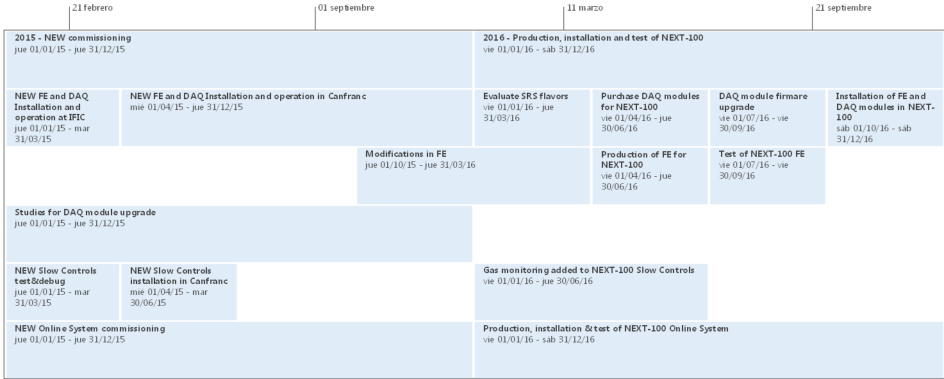
\includegraphics[width=0.99\textwidth]{img/ENF_CRONO.pdf}
%\end{center}
%\caption{\label{Fig:CronoEng} Cronogram for the ENG subproject. }
%\end{figure}
%
%\subsubsection*{Justification for the requested personnel}
%
%Two positions are requested with the following profiles:
%\begin{enumerate}
%\item	Electronics technician or BSc in Electronics Engineering, requested for three years of the Project (30 k\euro/year). Will carry out installation, maintenance, repairing and support of the front-end and DAQ interface electronics for NEW and NEXT-100, as well as the power supplies for sensors and electronics. Will also take part in the design and construction of small circuits (like filters or cabling). Will help in the commissioning phases and in the coordination of the electronic modules purchases and production and will carry out functional tests of the new units. Based in Valencia, will travel to LSC for installation and maintenance.
%
%\item Computer scientist/engineer (BSc or MSc), requested for four years (40 k\euro/year). Must be expert in Linux systems administration and Ethernet computer networks. Will configure, administer, maintain and support the different PC clusters (mostly running CERN Scientific Linux) in the DAQ, Online and Offline systems. Will configure the DATE environment for the DAQ system. Will scale these systems according to specific needs (like the upgrade from NEW to NEXT-100). Will manage the data storage. Will carry out R\&D programs to enhance performance. Construction and commissioning. Based in Valencia, will travel to Canfranc for installation and maintenance.
%
%\end{enumerate}
%

\paragraph{Objectives of the CALREC subproject.}

The specific objectives of this subproject are:
\begin{enumerate}
\item {\bf Photo-detectors calibration system}. Design, construction, commissioning and operation of a calibration system to estimate the gain and noise of the SiPM and PMT sensors of NEW and NEXT-100. 

\item {\bf Energy calibration system}. Design, construction, commissioning and operation of an energy calibration system with external radioactive sources for NEW and NEXT-100.

\item {\bf Position calibration system}. Design, construction, commissioning and operation of a position calibration system using the X-rays produced by a $^{83}$Rb source. 

\item {\bf Xenon additives}. Development of a dedicated testing system to evaluate additives capable to improve the performance of pure xenon. 

\end{enumerate}


\paragraph{Objectives of the BATA subproject.}

The BATA subproject will focus on the R\&D program needed to clearly establish the feasibility of tagging (e.g., detecting) the barium (Ba$^{++}$) ion produced in the double beta decay of xenon. 
%Demonstrating that an efficient detection of barium is possible in an \HPXE\ would imply that the NEXT technology could be upgraded to the ton scale while at the same time reducing the background by two or more orders of magnitude, resulting in a virtually background-free experiment with enormous possibilities of hitting a discovery. 

The BATA program involves a set of proof-of-concept experiments. It also proposes the development of a 4.1 $\mu$m laser, needed for the deshelving of the metastable state D. An attractive feature of such a laser is its wide range of scientific and technological applications. CLPU is especially well suited to develop the technology. It is important to notice that, although NEXT deals with particle physics, the BATA subproject deals with the part of NEXT directly related with the spectroscopy of Ba ions and the lasers needed in order to do and improve that spectroscopy. This is a subject clearly related to atomic physics and fits very well with the scientific background of the PI of the subproject. The different objectives of this subproject are, therefore:

\begin{enumerate}
	\item \textbf{Ba ions generation, phase 1}. Proof-of-principle experiment with Ba ions generated by means of an electrical discharge.
	
	\item \textbf{Ba ions generation, phase 2}. Proof-of-principle experiment with Ba ions generated by an ion source.	
	
%	\item \textbf{Proof of principle experiment with Ba ions generated by an ion source and with a magneto trap.}	
% In order to better control the experimental conditions, we will repeat the experiment but with the ions now confined in a magnetic trap. This trap will allow us to have an excellent degree of control over the experimental conditions and to approach the conditions that can be expected in the NEXT experiment. For instance we will carry out different measurements comparing the collected fluorescence signal as a function of the pressure of the Ba$^+$ ions and the pressure of the surrounding environment. These measurements are mandatory because the population dynamics is very sensitive to pressure, i.e., to collisions. 
%	
	\item \textbf{D state deshelving}. A likely scenario is that the collisional induced decay between the metastable state D and the ground state S is either not effective or too slow for obtaining an appreciable fluorescence signal. In this situation the population is trapped in the metastable state D and the fluorescence cycle can not be closed. To avoid this difficulty, deshelving the D state may be needed. A proof-of-principle experiment with an additional laser for deshelving the D state will be performed.

\item \textbf{Development of a state-of-the-art 4.1\,$\mu$m laser}. The laser needed for deshelving the D state must have a wavelength of around 4.1\,$\mu$m. While small commercial laser systems exist in this range (we will purchase one of them for the experiment described in the previous paragraph), no commercial system will satisfy the conditions of power and stability needed for a real BATA experiment. Furthermore, such a laser, already well in the infrared region, has many potential applications.

\end{enumerate}

%\subsubsection*{\BATA\ subproject: Resources}
%
%For the successful development of this subproject, CLPU will provide the required human and technological resources. CLPU is the centre of reference in Spain regarding laser technology, and takes active part in several international and national projects. The leader of this subproject will be Alicia V. Carpentier who has a well recognised international trajectory in laser-matter interaction. Moreover, {\bf CLPU considers this project of high priority and consequently will offer the collaboration of all the scientific department} consisting of a multidisciplinar team with broad experience in laser technology and development, and laser-matter interaction. 
%
%Furthermore, CLPU will support this project with some of the already operating laser systems in its installation. This is extremely important because such systems usually cost of the order of several hundreds of thousand euros. The human resources needed to operate the laser systems will be provided by CLPU as well. For the construction of the ion source, and taking into consideration the specific requirements of this development, we will apply for an \emph{EXPLORA tecnología} in the 2014 call. 
%
%The budget of this subproject will be dedicated to: a) purchase small equipment for the proof-of-principle experiments; b) purchase a small commercial infrared laser for the initial deshelving experiment; c) develop a state-of-the-art, high power, very stable infrared laser to be used in a large system. It is important to insist that such a laser has many possible applications given the fact that its wavelength is not absorbed by the atmosphere as it lies in what is called the infrared atmospheric window.
%
%
%\subsubsection*{BATA subproject: schedule}
%
%
%


\subsubsection*{Metodolog\'ia / Methodology}

%4. El detalle de la metodologia propuesta en cada uno de los subproyectos participantes
The specific objectives of all the subprojects are integrated in the NEXT Project Management Plan (PMP). The PMP coordinates the construction of the NEW and NEXT-100 detectors. It is under the direct supervision of the Spokesperson (SP) and the Project Manager (PM). The PM of NEXT is Dr. I. Liubarsky, part of the IFIC group. 

The PMP defines a set of Working Packages (WP) and follows the progress of each one, monitors deliverables and deadlines and keeps track of invested resources including personnel. It also identifies potential show-stoppers and synergies (and possible conflicts) between the different projects and optimises the sharing of resources. 

%Figure \ref{fig.Gantt} shows an example of the Gantt chart for the whole NEW project, up to installaton at the LSC. 

%The objectives defined for the different sub projects match the various WP in the PMP, as can be seen in Figure \ref{Fig:PMP}. 

The methodology of each WP includes: a) the definition of the associated tasks; b) the identification of the resources needed; c) the temporal organisation of the tasks; d) the definition of milestones and the deliverables associated to them; e) the relations with other WP. Each WP has a leader, which reports directly to the PM. The progress of each WP is reviewed on a weekly basis. Milestones and potential showstoppers are discussed, and the tracking charts updated if needed. The PMP is reviewed every six months by the LSC scientific committee.  
\paragraph{Methodology of the COORD subproject.}

The first objective of the COORD subproject is the {\bf construction of the NEW detector}. The construction of NEW will involve:

\begin{enumerate}
\item {\em Construction of the NEW and NEXT-100 pressure vessels}.
The NEW and NEXT-100 pressure vessels were designed to withstand pressures in excess of 20 bar, and to operate with negligible losses at 15 bar. They are built using a 316Ti alloy of low activity. 
The design was a collaboration between IFIC and LBNL groups. They have been manufactured by several Spanish companies (TRINOS, MOVESA and ACYM). They will be shipped to LSC in Q1'15 and commissioned during Q2'15. 

\item {\em Construction of the NEW and NEXT-100 field cage (NFC)}
The NEW and NEXT-100 field cage produces an uniform electric ($\sim$ 300 V/cm) field inside the  detector that drifts the ionisation electrons to the anode, where they are further accelerated in the electric field produced between a pair of transparent grids, called the electroluminescent (EL) grids. 

The main body of the field cage is a high density polyethylene (HDPE) cylindrical shell with a 2.5\,cm wall thickness (Figure \ref{fig:FC}, left, shows the NEW field cage body).  The drift region consists of radiopure  copper strips connected with low radioactivity resistors.  The light tube consists of thin sheets of teflon, coated with tetraphenyl butadiene (TPB). The role of the TPB is to shift the UV light produced in xenon to the blue region (PMT and SiPMs operate best in this region, around 450 nm).  A high-voltage feedthrough (HVFT) in the cathode and another one in the anode, allow the definition of the voltages (Figure \ref{fig:FC}, right). The cathode HVFT is designed to withstand up to 100 kV, and the HVFT of the anode to withstand up to 40 kV. The design of the HVFT, identical for NEW and NEXT-100 improve those that were built for DEMO by the Texas A\&M group. The field cage and grids of NEW and NEXT-100 are also identical, to a scale 1:2. The grids use a stainless steel mesh with pitch 0.5 mm and wire diameter 30 microns, which results in an open area of 90\%. 

The construction of FC for NEW is currently under way (Q4' 2014). The HDPE body has been fabricated by the spanish company AIMPLAS. The HVFT and the grids have been manufactured at Texas. The  NFC will be tested at IFIC before shipping and installation in the LSC in Q1'15. The field cage will be commissioned in Q2'15. System commission, together with the rest of the systems will occur during Q3'15 and Q4'15.

\item {\em Construction of the NEW and NEXT-100 energy plane }
In NEW (NEXT-100) the energy measurement will be provided by the detection of EL light via PMTs, which will also record the scintillation light needed for $t_0$. Those PMTs will be located behind a transparent cathode.

A total of 12 (60) low-background, high-QE PMTs, model R11410-10 from Hamamatsu (Figure  \ref{fig:sensors}, mid panel) covering 32.5\% of the cathode will be deployed for NEW (NEXT-100) . The R11410-10 are large tubes, with a 3'' photocathode and low levels of  activity of the order of 1 mBq per unit in the Uranium and Thorium series. The PMTs are sealed into individual pressure resistant, vacuum tight copper enclosures (called PMT cans) coupled to 
sapphire windows, coated with ITO (for electrical conductivity) and TPB (Figure  \ref{fig:sensors}, right panel).

The NEW energy plane (NEP) is currently (Q4'15) under construction at IFIC. The ``PMT can'' design have been validated and production of the parts has started. The NEP will ship to LSC during Q1'15. It will be commissioned in Q2'15. System commission, together with the rest of the systems will occur during Q3'15 and Q4'15.

\item  {\em  Construction of the NEW and NEXT-100 tracking plane (NTP)}:
In NEW and NEXT-100 the tracking function is provided by a plane of multi-pixel photon counters (SiPMs) operating as a light-pixels and located behind the transparent EL grids. They are mounted in flexible radiopure Kapton Dice Boards (KDB). Each KDB hosts 64 SiPMs (Figure  \ref{fig:sensors}, left panel) .The NEW (NEXT-100) tracking plane will deploy 28 (112) such KDBs. 

The NTP is currently under construction at IFIC (Q4'14). The KDB production has been validated and prototypes have demonstrated excellent performance. The NTP will ship to LSC during Q1'15. It will be commissioned in Q2'15. System commission, together with the rest of the systems will occur during Q3'15 and Q4'15. 

\end{enumerate}
 
%%%%%%

The main objective of the COORD subproject is the {\bf fabrication of NEXT-100}. The construction will start in 2016 and will take 12 months. This fast schedule is possible thanks to several factors:
%
\begin{enumerate}
\item {\em Reuse of infrastructures}: the platform, pedestal, lead castle, gas system, clean tent, radon suppression system, online computing, slow controls and calibration hardware and procedures are common to NEW and NEXT-100 and will be extensively tested during NEW operation, thus ready for NEXT-100 phase.
\item {\em Early construction of pressure vessel}: The pressure vessel is a critical system, since it has to operate underground, at high pressure and with negligible losses. Designing, constructing and certifying it takes a long time. Luckily, this fact was understood at an early stage in the development of the project and the NEXT-100 pressure vessel (see Figure \ref{fig:PV}) was constructed during 2014, and has been tested and certified at the same time than the NEW pressure vessel. 
\item {\em Scalability of the field cage}: Some of the most delicate subsystems of the field cage (such as the HVFT) have been designed and tested to be operative in NEXT-100 (for example the HVFT in the cathode holds up to 100 kV voltage, while the nominal operation of NEXT-100 is 50 kV). The NEXT-100 field cage body will be constructed by the same company (AIMPLAS) that has built the NFC body, reusing the tools and procedures that have been put together for the task. This also applies to the construction of the EL grids. 
This makes possible to foresee an early assembly of the NEXT-100 field cage, in Q2'16, allowing for ample time for testing and debugging.

\item {\em Production chains for the energy and tracking planes}. The energy and tracking planes are composed of individual modules (PMT cans in the case of the energy plane, KDBs in the case of the tracking plane), mounted to supporting plates and connected to electronics. The structure of the systems is the same (as seen in Figure \ref{fig:EnergyPlane}). The number of modules (cans and KDBs) is larger in NEXT-100 (by about a factor 5), but, very importantly, the construction procedure is the same. This allow us to set {\em production chains}, PC, of both PMT cans and KDBs. The PCs will be extensively exercised during the construction of NEW, and are expected, therefore, to run smoothly during NEW construction.  

The production chains should be able to produce 20 PMT cans and 30 KDBs a month. We therefore, expect that the modules will be ready in Q1'16. Shipping and cleaning will take the best part of Q2'16. The systems should be assembled at the LSC in Q3'16, allowing for testing and debugging during Q4'16.
\end{enumerate} 
\paragraph{Methodology of the ENG subproject.}

\begin{figure}[h!]
\begin{center}
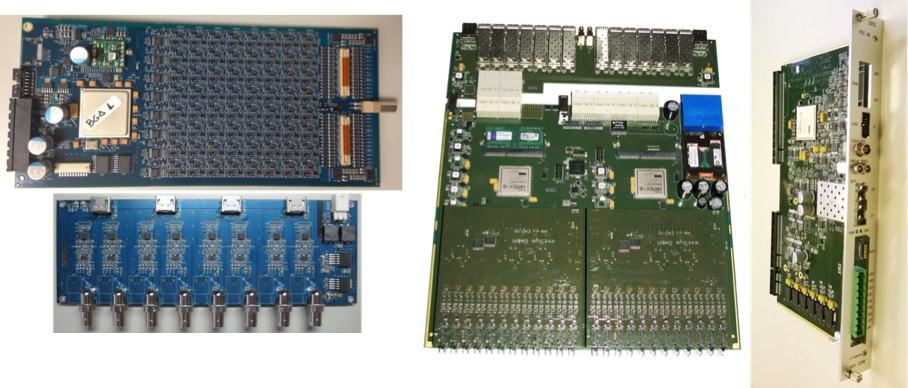
\includegraphics[width=0.7\textwidth]{img/Electronics.jpg}
\end{center}
\caption{\label{Fig:FEE}\small Left: Front-end boards for SiPM (top) and PMTs (bottom) for NEW and NEXT-100. Right: SRS FEC modules in ATCA form factor (left) and “SRS classic” flavour (right).}
\end{figure}

The ENG subproject is responsible for the {\bf front-end electronics} for the PMTs and the SiPMs for NEW and NEXT-100. Critical items include:
%
\begin{enumerate}
\item	{\em Commissioning NEW front-end electronics in 2015}. As an outcome from two previous projects (CUP and FIS2012-37947-C04-04), the front-end electronics for both the PMT plane and the SiPM plane in NEW are available. The former is already being used in NEXT-DEMO while the latter, an evolution from the NEXT-DEMO electronics, exists as prototype boards and will be available in adequate quantities by the end of 2014. Required cabling, power supplies and mechanical structures have already been purchased.
These electronics will be tested at IFIC in Q1’15 and at the LSC in Q2’15. A study on reliability, performance and signal noise will be carried out during the commissioning phase, resulting either on the final validation of the current designs or on a proposal for changes. In this case, the changes will be carried out in Q4’15 and Q1’16.

\item {\em Production, installation and test of NEXT-100 front-end electronics in 2016}. Lessons learnt with NEW commissioning and initial operation will lead to a document on recommendations for installation and operation of electronics in NEXT-100. The specificity of LSC in terms of grounding and power distribution in the experimental area, together from noise in the power lines and generated by neighbouring experiments, will determine the required noise-reduction techniques (mostly ground connections and ad-hoc filtering). After completing the eventual modifications in the front-end modules (Q1'15), production for NEXT-100 in Q2’16, and Q3'16, module test in Q4’16 will complete the 2016 work plan.

\item {\em Commissioning and Operation of NEXT-100 front-end electronics in 2017}. Potential problems found after installation in a detector of the size of NEXT-100 will be addressed. Front-end firmware may require fine adjustments to (1) ease later energy measurement and tracking algorithms and (2) adjust the trigger algorithms as specified for the different physics campaigns. Commissioning is scheduled for Q1-Q2’17. Operations start on the second half of the year.
\end{enumerate}

%%%%%%%%%%%%%%%%%%%%%%

The second objective of this subproject is the design, fabrication and commissioning of the {\bf data acquisition modules} for NEW and NEXT-100. The following main tasks have been identified:

\begin{enumerate}

\item	{\em Commissioning NEW DAQ interface electronics in 2015}. The DAQ interface modules for NEW and NEXT-100 are also available in two flavours: “classic” SRS modules (19” Eurocard form factor, available from CERN Store) and industry-standard ATCA SRS modules. NEW DAQ will use in a first stage modules from both flavours.

These electronics will be tested at IFIC in Q1’15 and at LSC in Q2’15. A study on reliability and performance will be carried out during the commissioning phase, allowing to choose the best solution for NEW and NEXT-100. 
%A third option, a new SRS solution for very-close-to-detector readout codenamed OC-Box, which is to be developed in collaboration with RD51 and intended as an upgrade for NEXT, will be evaluated in 2015 as a future upgrade. It is based on newer FPGA technology and can replace current FEC modules.

\item	{\em Production, installation and test of NEXT-100 DAQ electronics in 2016}. Lessons learnt with NEW commissioning and initial operation will lead to a decision to go for “classic” or ATCA SRS flavor. Purchases for NEXT-100 in Q2’16, module test and firmware upgrade in Q3’16 and installation in Q4’16 will complete the 2016 work plan.

\item	{\em Commissioning and Operation of NEXT-100 DAQ electronics in 2017}. DAQ performance and functionalities will be verified and adjusted to meet final NEXT-100 requirements. DAQ firmware may require some modifications to (1) ease energy measurement and tracking algorithms and (2) adjust the trigger algorithms as specified.

%\item	NEXT-100 operation in 2018. The DAQ requires no maintenance during operation other than module replacement due to damage or malfunctioning. Placed outside the lead castle in 19” racks next to the front-end modules, the DAQ electronics are easily accessible.

\end{enumerate}

%%%%%%%%%%%%%%%%%%%%%%

Concerning the third objective of the ENG subproject, the {\bf slow controls system} for NEW and NEXT-100, six subsystems or partitions have been defined: (1) high-voltage sources for PMTs, (2) low-voltage sources for SiPMs and electronics, (3) high-voltage for grids, (4) gas system status -getters, pump and gas recirculation-, (5) a group of temperature and pressure sensors and (6) the main control panel (with cameras and status overview). Partitions are interconnected via Ethernet. Basic functionalities for all subsystems have been implemented in 2014. The Slow Controls for NEW will be completed in Q4’14, tested and debugged in Q1’15 and installed in LSC in Q2’15.

%Power supplies for PMTs and SiPMs are directly controlled to Ethernet. Power supplies for the electronics are controller from a PC via USB, being this PC connected to Ethernet. The other subsystems are controlled via a National Instrument’s Compact-RIO chassis with Ethernet link, embedded in a so-called “Slow Control Box”, which includes relays and connections. A LabView software application will be used for the main control panel.

%\begin{enumerate}
%\item {\em Design, production and commissioning NEW slow-controls in 2015}. The Slow Controls for NEW will be completed in Q4’14, tested and debugged in  Q1’15 and installed in LSC in Q2’15.

%\item {\em Production, installation and commissioning of NEXT-100 slow-controls electronics}. Monitoring the gas subsystem will be an addition to the Slow Controls for NEXT-100 in 2016.
%\end{enumerate}

%%%%%%%%%%%%%%%%%%%%%%

Finally, the ENG subproject is respnsible for the {\bf online system} for NEW and NEXT-100. The Online System for NEW comprises the following subsystems: (1) Data Storage, (b) Backup Storage, (c) Pre-processing and (d) Online Monitoring. The DAQ System (a PC farm comprising Local and Global Data Concentrators) produces approx. 30 MByte/s in NEW, which are stored into the NEW Data Storage (up to 8 servers with 8 disks each for up to 65 TByte). The Data Storage has power redundancy and multiple network cards per PC for enhanced reliability. Long-term data selected by the Offline System are stored into the Backup Storage (composed of a server PC and a tape server using 1.5 TByte tapes). The Pre-processing comprises two servers which read event data from the Data Storage and apply a format for later offline processing. Finally, a server in the Online Monitoring is used to gather statics, measure performance, find out bottlenecks and check the health of the different subsystems. A 1-Gb Ethernet switch interconnects the PC servers in the Online System, using virtual LANs to separate different data flows.
Backup Storage, Pre-Processing, Data Storage and Online Monitoring have been tested.
 
\paragraph{Methodology of the CALREC subproject.}

The {\bf gain and noise of the PMTs and SiPMs} will be calibrated using two sets of 400 nm LEDs located on the tracking and energy planes. The gain and noise of SiPMs and PMTs will be calculated for each sensor fitting their single photo-electron response. This procedure has been demonstrated in DEMO for the calibration of the energy plane\footcite{Lorca:2014sra}. In NEW, we will apply it also to the calibration of the last generation SiPMs deployed in the tracking plane, which have a much lower dark current than those deployed in DEMO (100 kHz per device to be compared with several MHz) and are, therefore, capable of counting single electrons.

The CALREC subproject is also responsible for the {\bf energy calibration of the NEW and NEXT-100 detectors}. The energy scale and energy resolution has been measured in DEMO using \NA\ and \CS\ radioactive sources\footcite{Alvarez:2012nd,Alvarez:2013gxa}. A fit to the photoelectric spectrum of the gammas interacting in the gas yields a gaussian distribution whose mean value sets the energy scale, while the RMS (or, as is customary in the field, the full width half maximum, FWHM) defines the resolution (see Figure \ref{fig.ERES}). In DEMO, the energy resolution has been measured at relatively low energies (511 and 662 keV), and the resolution in the region of \Qbb\ has been extrapolated using the scaling law $\delta E \propto 1/\sqrt{E}$, which has been demonstrated to hold well in the range between X-rays (35 keV) and \CS\ interactions (662 keV). 

The energy calibration in NEW and NEXT-100 will use the photo-peak of the 2.6 MeV gamma from a \Tl~  source to measure the energy resolution very near \Qbb. In addition, \NA\ and \CS~ sources will be used to calibrate the energy scale at  511 keV, 662 keV and 1.3 MeV. Adding the low energy point obtained with xenon X-rays (35 keV), we will be able to calibrate the energy in the full scale relevant for the experiment. The procedure is well understood from DEMO. The main novelty in NEW and NEXT-100 is the mechanical system, currently being designed, that will allow us to introduce and withdraw the radioactive sources from the chamber using special access ports. The calibration system will be built at US in Q1-Q2'15 and installed at the LSC in Q3'15.

The \TL\ source also produces double electrons (double escape peak of \TL) with an energy of 1.6 MeV, not very far from \Qbb. Such double electrons, together with single electrons at 1.3 MeV from a \NA\ source can be used to measure the single and double electron selection efficiency from the data themselves (recall that the selection of \bb\ events require a positive double-electron identification).

Calibration runs will be taken periodically. Typically a long run per month should be enough, but the exact procedure will be defined as part of the commissioning process of NEW and NEXT-100. 

The third objective of the CALREC subproject is the design, construction, commissioning and operation of a {\bf position calibration system}. Position calibration is needed to correct for the bias on the energy introduced by the geometry of the chamber. As demonstrated using NEXT-DEMO data\footcite{Lorca:2014sra}, PMTs detect less light for events outside the central region of the detector. In DEMO, X-rays from xenon (35 keV) have been used to correct the position dependence of the energy. The procedure takes advantage of the fact that X-rays behave like point-like sources. One can, therefore, reconstruct their position in the detector (using the tracking plane) and measure their apparent energy (using the energy plane). The apparent energy differs from point to point, and thus one forms a weight matrix  (obtained normalising to the energy measured in the center of the camber) that is used to correct point-by-point the energy measured in the chamber.

Computing the energy weight matrix requires many X-ray interactions {\em in all the chamber}. In DEMO, those X-rays were produced by de-excitation of the gas when using conventional (\NA, \CS) radioactive sources. The statistics that can be collected with such a procedures is limited, however, and both NEW and NEXT-100 require much larger statistical samples.

We have proposed, therefore, the use of X-rays from Krypton, a technology demonstrated in liquid xenon detectors\footcite{Kastens:2009rt}. A source of $^{83}$Rb
decays to the metastable state  $^{83}$Kr$^m$~ with a half-life of 86.2 days. The
$^{83}$Kr$^m$~subsequently decays via emission of 3.1 keV and 9.4 keV conversion electrons with a half-life of 1.83 hours. Thus, no long-lived isotopes are introduced in the xenon gas, and the fact that krypton is itself a noble gas guarantees no problems of chemical purity.  

The $^{83}$Rb~source is infused in a zeolite which is introduced in the gas system by adding a simple VCR cross (the zeolite itself is a small piece of 2 grams mass). The side arms of the the cross allow gas to flow through the chamber and a filter prevents the introduction of the zeolite into the gas system. The top arm of the cross allows the injection of the $^{83}$Rb~in the form of aqueous solution. A typical injection of 10 $\mu$l, discharged into the zeolite via a syringe yields 700 nCi of $^{83}$Rb. The rubidium itself stays attached to the zeolite, while the $^{83}$Kr$^m$~reaches an equilibrium rate in the range of several tens of kBq, enough to produce a very large statistical sample for calibration. Xenon is then circulated through the cross during several minutes, carrying the radioactive krypton gas with it.  

The rubidium source will be procured by the US group in 2015. The system will be commissioned in Q4'15 or Q1'16, depending of the progress of the energy calibration system. Extensive analysis of rubidium data during 2016 will yield the weight matrix for NEW. The same procedure will then be repeated for NEXT-100. 

%\begin{figure}
%\begin{center}
%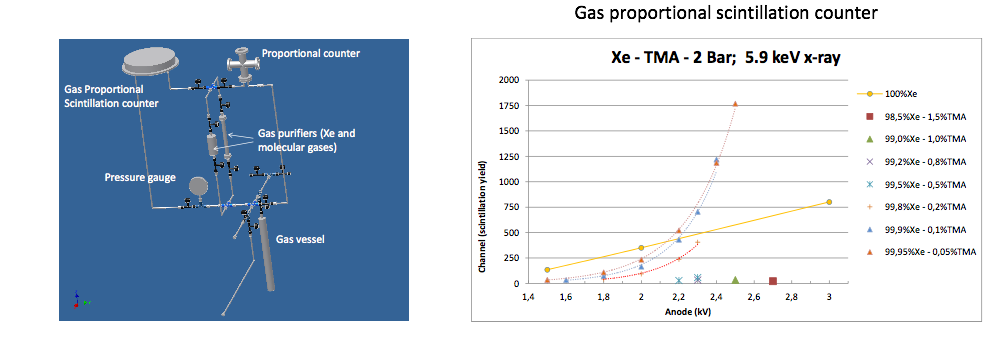
\includegraphics[width=0.99\textwidth]{img/TMA.png}
%%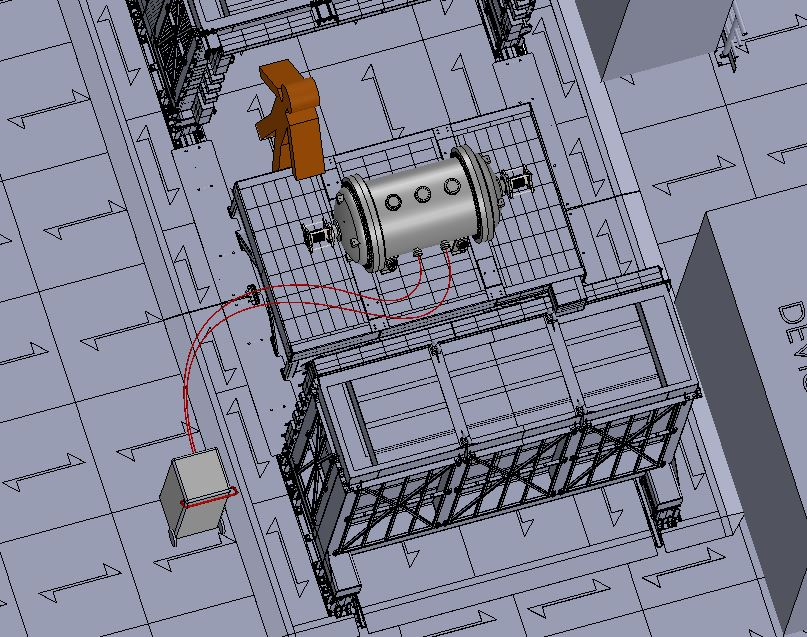
\includegraphics{img/CALIB_LSC_sources.jpg}
%\caption{\small Left: a small experimental setup to test gas mixtures. Right: initial results on scintillation yield obtained with the setup.}
%\label{fig:additives}
%\end{center}
%\end{figure}
%
%Finally, the ENG subproject will also be responsible for developing a dedicated testing system to evaluate {\bf additives capable to improve the performance of pure xenon}. The US will lead the R\&D focused in the studies of additives (for example TMA, trimethylamine) mixed with xenon, which will be carried out in collaboration with the Portuguese groups of Coimbra and Aveiro. These additives reduce the electron diffusion, which translate into a more confined trajectory.  In addition the scintillator light has  a 300 nm wavelength, easier to detect than the one of xenon (170 nm). Furthermore, some of the additives (including TMA) are capable of transferring the charge from the Ba$^{++}$~ion produced in a \bb\ xenon decay to
%the Ba$^{+}$~ion which can be tagged (e.g., $Ba^{++} + A \rightarrow Ba^{+} + A^{+}$) where $A$~is the additive. 
%
%Figure \ref{fig:additives} (left) shows a small setup to measure the effect of additives in the gas. A preliminary result using this setup shows that very small concentrations of TMA result in a very large increase of the scintillation yield. Larger concentrations, on the other hand, quench the yield. We plan a systematic campaign of measurements using several additives (TMA, TEA,CH$_4$~CF$_4$~and others) that will study at depth the effect on scintillation yield, attachment and resolution of different mixtures (including very small concentrations), and as a function of pressure. This campaign requires a modification of the setup to allow operation at higher pressure, as well as monitoring systems to control very small concentrations of the additive. 
%
%The initial R\&D will be done with the simple setup already available, at pressures of up to 2-3 bar. During 2015, we will characterise different additives and choose the most suitable ones for NEXT. In 2016, the setup will be upgraded to take higher pressures and further studies will be performed up to operating pressures of 10-15 bar. In 2017 we plan to operate the DEMO detector with the chosen additive, to characterise the performance of the mixture in a large system. We will use our calibration protocol, described above, to measure electron tracks and energy resolution at different energies, to quantify the potential improvements of the mixture. 
%
%In addition, we will carry an experiment, in coordination with the \BATA\ program  to measure the charge transfer $Ba^{++} + A \rightarrow Ba^{+} + A^{+}$, where $A$~is the chosen additive. The exact schedule of such an experiment will depend on the overall \BATA\ program, but we expect that it will be performed in 2016. 
\paragraph{Methodology of the \BATA\ subproject.}

In a first round of experiments we will excite resonantly the S$\leftrightarrow$P transition of {\bf Ba$^+$ ions generated by an electrical discharge} between two barium electrodes and will collect the fluorescence signal of the P$\rightarrow$D transition. Although this generation method is not ideal because several species different from Ba ions will be generated (e.g., BaO molecules or clusters), it does not need a major technological development. 

\begin{figure}
\begin{center}
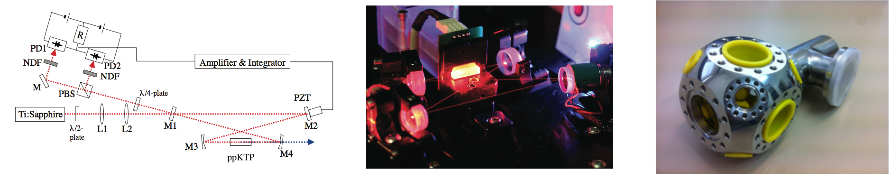
\includegraphics[width=0.99\textwidth]{img/blueLaser.png}
%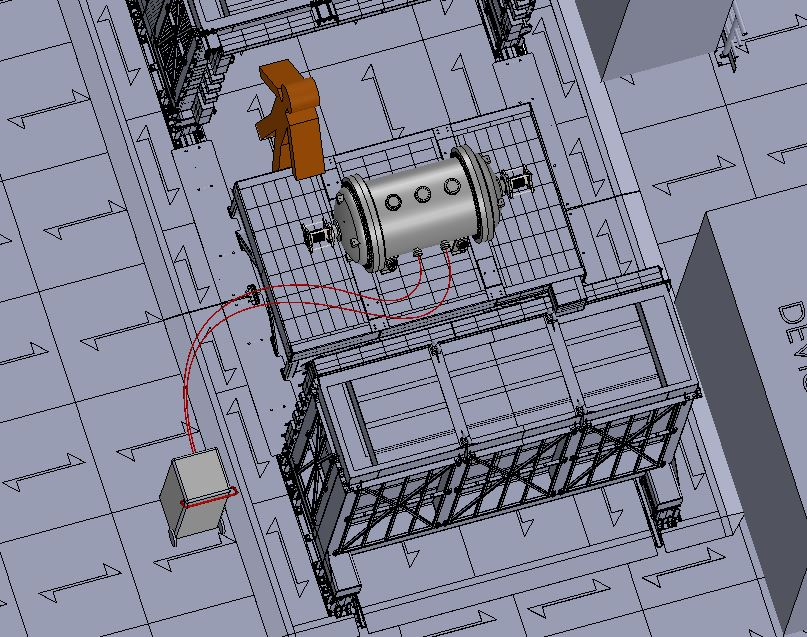
\includegraphics{img/CALIB_LSC_sources.jpg}
\caption{\small Left: experimental set-up for resonant frequency doubling of a 
Ti:Sapphire laser using ppKTP. Right: the chamber for the proof-of-concept experiments, built at IFIC, and ready to be installed at CLPU.}
\label{fig:chamber}
\end{center}
\end{figure}

The laser source needed to resonantly excite the $Ba^{+}$ ions must have a wavelength of 493.5\,nm, not available in commercial lasers. The laser source will, therefore, be produced at the CLPU, optimising a tunable Ti:sapphire laser at 987\,nm to obtain a second harmonic generation (SHG) at 493.5\,nm, see Figure \ref{fig:chamber}. This setup allows the tuning of the wavelength and controls the bandwidth of the laser, a necessary feature to precisely tune it to the transition frequency (e.g. to correct for pressure broadening and other effects). The IFIC group, on the other hand, has fabricated the test chamber needed for the experiments (see Fig.~\ref{fig:chamber}). 

It is expected that this initial set of experiments will provide valuable information about the population dynamics in Ba$^+$ ions, and the influence of the different homogeneous and inhomogeneous broadening mechanisms. 

The second objective of the \BATA\ subproject is to {\bf generate Ba ions by an ion source}. For this objective, in order to get a better approximation of the final conditions of NEXT experiment a source of ions will be designed and constructed at the CLPU. This ion source will be based on selective ionisation and mass spectrometry techniques, and it will allow an efficient selection of the desired target species (e.g, $Ba^{+}$~and $Ba^{++}$). With this setup we will be able to study the recombination process Ba$^{++}\rightarrow$Ba$^{+}$ and decide whether it can be induced by collisions with xenon atoms, or whether it requires an additive (see discussion in the objectives of the CALREC subproject). Depending on the results of the experiment, a magnetic trap can be added to improve the experimental conditions. 

The third objective of the \BATA\ subproject is to perform a proof of principle experiment with an {\bf additional laser for deshelving the D state}. Our approach will be to use a second laser to induce a two photon transition (one photon is forbidden by selection rules, between the states D and S, see Fig.\,\ref{fig.BATA}). 	

The fourth objective of the \BATA\ subproject is the {\bf development of a state-of-the-art 4.1\,$\mu$m laser}. There are only a few laser systems that generate laser emission in the mid-infrared (MIR, from 2 to 10\,$\mu$m). There are lasers that emit in discrete wavelengths as gas lasers ($CO_2$, Xe-HE, He-Ne), chemical lasers (Hydrogen Fluoride, Deuterium Fluoride) and Dye lasers by Raman Shift. All these systems are large and complex, emit in relative low power and involve the use of dangerous materials (chemicals, flammable gases and/or carcinogenic powders). 

\begin{figure}[h!]
\begin{center}
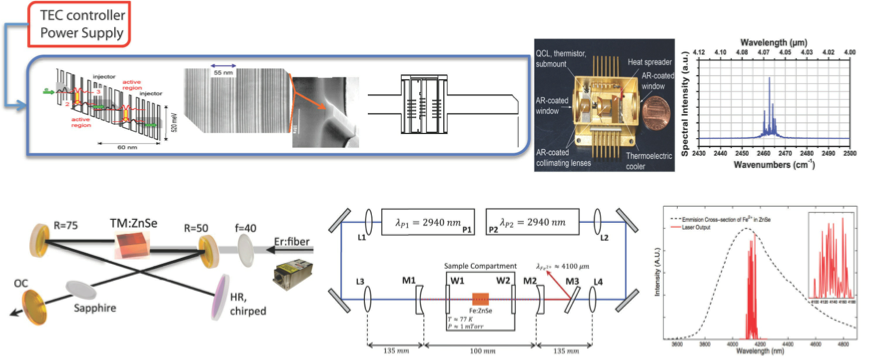
\includegraphics[width=0.99\textwidth]{img/MIR.png}
\end{center}
\caption{\label{Fig:MIR}\small Top: band theory of a quantum cascade laser (QCL), semiconductor material with physical bands and first device with laser spectrum at MIR. Bottom: schematic view of the TM:ZnSe laser design (two potential configurations with Er pumping laser) with potential tunable laser curve and free running emission. All MIR optics are made of CaF2, ZnSe and AR-coated at 2940 - 5000 nm.}
\end{figure}

A much more interesting alternative to reach the desired MIR wavelength is the use of an optically pumped solid state laser (OPSSL) system, by means of a specific doping of crystals with metal transition ions, see Fig.~\ref{Fig:MIR}. Wavelengths of 2 and 2.9\,$\mu$m are available with $Tm^{3+}$, $Tm^{3+}$-$Ho^{3+}$ and $Er^{3+}$ active ions in crystalline matrices. Recent developments involve doping with $Cr^{2+}$ and $Fe^{2+}$ ions. This approach should allow us to develop a laser system that emits in a broad range: 2.1 to 3\,$\mu$m and 3.7 to 5\,$\mu$m, respectively. Another option is to work with quantum cascade semiconductor systems potentially available from 3.8 to 9.5\,$\mu$m in a discrete range, i. e.  not only continuously. 

To develop a laser system around 4.1\,$\mu$m we need to study and evaluate the best optical parameters of some materials (crystalline matrices or semiconductors) that can be used as active laser materials.  This will allow us to design a laser cavity with the appropriate  optical components and devices (these should work in the MIR region). It will also allow us to maximise the efficiency of the laser system. The cavities are different for optically pumped systems (the case of crystals doped with $Cr^{2+}$ o $Fe^{2+}$) or for electrically pumped systems (as the quantum cascade semiconductors). These cavities can be 2-, 3- or 4- folded mirror configurations depending on the advantages observed during the design using optical and numerical software. The characterisation of the laser emission and other related parameters will allow us  to improve the laser system to use in the NEXT experiment.  

\subsubsection*{Infraestructuras, equipamientos y propuesta de co-financiaci\'on (equpamientos y fungible) / Infrastructures, equipment and co-funding request (equipment and fungible)}

%5. La descripción de los medios materiales, infraestructuras y equipamientos singulares a disposición de los participantes que permitan abordar la metodología propuesta.
% Los objetivos específicos de cada uno de los subproyectos participantes, enumerándolos brevemente, con claridad, precisión y de manera realista (acorde con la duración prevista del proyecto).
%
% En los subproyectos con dos investigadores principales, deberá indicarse expresamente de qué objetivos específicos se hará responsable cada uno de ellos.
%

\subsubsection*{Equipment and Infrastructures: COORD, ENG and CALREC subprojects}

\begin{enumerate}
\item {\bf A state-of-the-art laboratory at IFIC}, developed and financed with funds from CUP. The DEMO detector is operating here. The laboratory includes a full gas system, infrastructures for vacuum and high pressure operation; high voltage and slow control systems; a full DAQ and computing system. 
\item {\bf A state-of-the-art laboratory electronics laboratory at IFIC}, which has made possible the very fast development of the tracking plane. 
\item {\bf A state-of-the-art electronics laboratory at UPV}, which has made possible the very fast development of the FEE and DAQ. Of particular interest is the collaboration of UPV with CERN, in the context of RD51 collaboration, one of the main reasons why NEXT has been declared CERN recognised experiment.
\item {\bf Computation resources at the US}, where there is a large cluster (Tier2 class) 
for distributed LHCb analysis, with about 1500 processor cores. The NEXT experiment, through the PI of the CALREC subproject will have access to this cluster for Monte Carlo simulation and data reconstruction. 
\item {\bf Experimental laboratory at the US}, which 
includes a clean room (30 m$^2$ class 100000) with an automatic ultrasonic wedge bonding machine. This laboratory is ideal to set the gas-additive program to be carried out by US. 
item {\bf Infrastructures at LSC}, which include: a) working platform and seismic pedestal; b) lead castle; c) gas system; d) clean tent; e) radon suppression system. In addition, the LSC provided general support for the experiments. 
\item {\bf A state-of-the-art facility for radio purity measurements}, located at the LSC. 
\end{enumerate}

\subsubsection*{Equipment and Infrastructures: BATA subproject}

For the successful development of this subproject, CLPU will provide the required human and technological resources. CLPU is the centre of reference in Spain regarding laser technology, and takes active part in several international and national projects.  Moreover, {\bf CLPU considers this project of high priority and consequently will offer the collaboration of all the scientific department} consisting of a multidisciplinar team with broad experience in laser technology and development, and laser-matter interaction. 

The CLPU will provide a substantial part of the required infrastructure for the \BATA\ subproject, including.
 
 \begin{itemize}
    \item \textbf{Laboratory room for all the experiments:} The experiments will be fully performed at the CLPU laboratories.
    
\item \textbf{Workshop service:} The CLPU has a mechanical workshop capable of manufacturing high level designs. 

\item \textbf{Electronics workshop:} Offers general electronics service. 

\item \textbf{Auxiliary services:} KHZ amplified Ti:Saphire laser (Spitfire, Spectraphysics, 7 mJ 100 fs), laser micro-machining station, Optical and Scanning electron microscopes (ZEISS), plist DAQ services, vacuum equipment and optical equipment.   

%\item \textbf{Data acquisition equipment:} Three oscilloscopes up to 1 GHZ (Tektronix), data acquisition computer, 3 GHZ RF spectrum analyzer (Tektronix). 
%
%\item \textbf{Vacuum equipment:} Primary pumps, turbo-molecular pumps, general vacuum hardware.
%
%\item \textbf{Temperature control equipment:} Thermoelectrical chiller, 
%
%\item \textbf{Optical equipment (general, all for vis/nir):} Laser spectrum analyser (500-1500 nm), Laser spectrum analyser (1000-2600 nm), photodiodes (Ge, Si), ultra-fast photodiodes (300 ps), CCD cameras, two Laser Beam profilers (Gentec), optical autocorrelator (up to 50 fs, sweep), home-made optical autocorrelator (single shot), alignment lasers (HeNe), shutters, chopper (Stanford), filters, lenses, mirrors, general optomechanics (posts, post holders, clamping forks, waveplates, diaphragms, etc), two infrared viewers (up to 1350 nm), optics and optomechanics (mirrors, lenses, LBO crystals for 800 and 1030 nm, posts, clamping forks, mounts, etc.)

\item \textbf{Lasers:} a 493.54 nm CW LASER: Pump laser (Coherent, Verdi G 20 W, 532 nm, CW); a tunable Ti:Saphire laser CW (750-1020 nm,  more than 4W).
%
%\item \textbf{Spectrometer (UV-VIS-NIR, MIGHTEX)}
%
%\item \textbf{Power and energy meters:} thermal and pyroelectrical. 

\end{itemize}



\paragraph{Budget requested for equipment and fungibles for NEXT: COORD, ENG and CALREC subprojects.}

The bulk of equipment and fungible requested by this co-ordinated project is devoted to the second phase of the experiment (the construction, commissioning and calibration of the NEXT-100 detector). 
 Infrastructures for the experiment are co-funded by CUP, LSC and the AdG/ERC, the costs of NEW are fully funded by the AdG/ERC grant, and the contribution of the USA groups also co-funds the construction of NEXT0100. 

\begin{table}[h!]
\begin{center}
\begin{tabular}{|l|c|c|c|c|c|c|}
\hline
 Item & Total Cost \euro & CUP	&USA &	LSC & AdG &	FIS2014 \\
 \hline
Infrastructures 	& 1.875.487 & 	131.702 & 	0 &	1.306.600 &	437.185 &	0 \\
NEW &	 689.189 & 	298.678 & 	0 &	0 &	390.511 &	0 \\	
NEXT0100	 &1.982.427 & 	368.203 &	413.457 &	0 &	0 &	1.200.767 \\
Computing (Online) & 0 & 0 & 	0 &	0 &	69.522 &	0 	\\
Slow Control & 18.271 & 	0 &	0 &	 &	0 & 18.271	\\
Calibration &	 0 & 	0 &	0 &	0 &	0  & 60.700	\\
 \hline
Total  NEXT &	 4.695.595 & 	798.583 &	413.457 &	1.306.600 &	897.218 &	1.279.738 \\
 \hline\hline
\end{tabular}  
\caption{Total costs of the NEXT project.}
\label{tab.TCOSTS}
\end{center}
\end{table} 

%\begin{table}[h!]
%\begin{center}
%\begin{tabular}{|l|c|c|c|c|c|c|}
%\hline
% Item & Total Cost \euro & CUP	&USA &	LSC & AdG &	FIS2014 \\
% \hline
%Gas System &	 434.177 & 	68.970 &	365.207 &	0 &	0 &	0 \\
%Platform and Castle	& 250.600 & 	0 &	0 &	0 &	250.600 &	0 \\
%Xenon (100 kg + 100 kg) &	 1.056.000 & 	0 &	0 &	0 &	1.056.000 &	0 \\
%Lead cleaning	& 44.582 & 	44.582 &	0 &	0 &	0 &	0 \\
%Cleaning equipment	& 18.150 & 	18.150 &	0 &	0 &	0 &	0 \\
%Clean tent	 59.878 & 	0 &	59.878 &	0 &	0 &	0 \\
%Radon suppression &	 5.400 & 	0 &	5.400 &	0 &	0 &	0 \\
%Radon monitoring &	 6.700 & 	0 &	6.700 &	0 &	0 &	0 \\
%Total infrastructures 	& 1.875.487 & 	131.702 &	437.185 &	0 &	1.306.600 &	0 \\
% \hline\hline
%\end{tabular}  
%\caption{Total costs of the infrastructures.}
%\label{tab.TINFRA}
%\end{center}
%\end{table} 
%
%\begin{table}[h!]
%\begin{center}
%\begin{tabular}{|l|c|c|c|c|c|c|}
%\hline
% Item & Total Cost \euro & CUP	&AdG &	LSC & USA &	FIS2014 \\
% \hline
%Pressure vessel &	 186.669 & 	 126.445 & 	 60.224 & 	 0 & 	 0& 0 \\ 
%Inner copper shield	& 32.670 & 	 0 & 	 32.670 & 	 0 & 	 0 & 	 0 \\ 
%Energy plane	& 131.271 & 	 88.572 & 	 42.699 & 	 0 & 	 0 & 	 0 \\ 
%Tracking plane	& 106.518 & 	 0& 	 106.518 & 0 & 	 0 & 	 0\\ 
%field cage	& 78.009 & 	 0 & 	 78.009 & 	 0 & 	 0 & 	 0 \\ 
%FE electronics	& 83.661 & 	 83.661 & 	 0 & 	 0 & 	 0 & 	0 \\ 
%DAQ and online &	 70.392 & 	 0 & 	 70.392 & 	 0 & 	 0 & 	 0 \\ 
%Total NEW&	 689.189 & 	 298.678 & 	 390.511 & 0 & 	0 & 0 \\ 
% \hline\hline
%\end{tabular}  
%\caption{Total costs of the NEW detector.}
%\label{tab.TNEW}
%\end{center}
%\end{table} 
%
\begin{table}[h!]
\begin{center}
\begin{tabular}{|l|c|c|c|c|c|c|}
\hline
 Item & Total Cost \euro & CUP	&AdG &	LSC & USA &	FIS2014 \\
 \hline
 Pressure vessel &	 277.332 & 	 102.850 & 	 0 & 	 0 & 	 0 & 	 174.482 \\ 
Inner copper shield &	 187.550 & 	 0 & 	 0 & 	 187.550 & 	 0 & 	 0 \\ 
Energy plane	& 625.318 & 	 265.353 & 	 0 & 	 123.420 & 	 0 & 	 236.545 \\ 
Tracking plane	&  287.237 & 	 0 & 	 0 & 	 102.487 & 	 0 & 	 184.750 \\ 
field cage	 & 184.344 & 	 0 & 	 0 & 	 0 & 	 0 & 	 184.344 \\ 
FE electronics	& 277.871 & 	 0 & 	 0 & 	 0 & 	 0 & 	 277.871 \\
DAQ and online &	 142.775 & 	 0 & 	 0 & 	 0 & 	 0 & 	 142.775 \\ 
Total NEXT-100	 & 1.982.427 & 	 368.203 & 	 0 & 	 413.457 & 	 0 & 	 1.200.767 \\ 
  \hline\hline
\end{tabular}  
\caption{Total costs of the NEXT-100 detector.}
\label{tab.TN100}
\end{center}
\end{table} 
 
Table \ref{tab.TCOSTS} summarises the total costs (equipment and fungible) of the project and details the funds requested. The amount is 1.279.738 \euro, which corresponds to 27\% of the equipment costs of the project and matches the external funds, profiled by AdG/ERC and USA contributions. 
Table \ref{tab.TN100} details the costs of NEXT-100 and the sharing of co-funding. 

\paragraph{Budget requested for equipment and fungibles for \BATA: BATA\& CALREC subprojects.}

\begin{table}[h!]
\begin{center}
\begin{tabular}{|l|c|}
\hline
 Item & Cost \euro  \\
 \hline
Laser and nonlinear crystals for MIR range &  9.000 \\
Optical pumping systems & 30.000 \\
Laser diode driver & 10.000  \\
Optical components &14.000 \\
Opto-mechanics: &10.000 \\
MIR detectors & 3.500 \\
Electronic components & 1.500\\
Fungible & 4.000 \\
  \hline
 Total &  82.000 \\
 \hline \hline
\end{tabular}  
\caption{Costs of the MIR laser.}
\label{tab.MIR}
\end{center}
\end{table} 

The BATA subproject requests co-funding to purchase the optical and opto-mechanical components needed to tune up the blue laser that will be devoted to the experiment (20.000 \euro) , and to develop the solid state MIR laser (82.000 \euro), see table \ref{tab.MIR}.  
The total requested in equipment and fungibles is 102,000 \euro.

The CALREC subproject will use existing infrastructures for the study of additives. Only fungible (gauges, filters, getters, piping) adding to 10,000 \euro\ and funding to purchase gas additives (10,000) \euro\ are requested to this project. 

\subsubsection*{Cronograma / Timetable}



\subsubsection*{Schedule/Cronogram of NEXT activities}

Table \ref{tab:schedule_new} and Table \ref{tab:schedule_n100} show the cronogram for the construction, commissioning and operation of the NEW and NEXT-100 detectors. The activities involve 3 of the 4 coordinated projects. 

\begin{center}
\begin{tabular}{| l | c | c | c | c |}
\hline
tasks & 2015 & 2016 & 2017 & 2018 \\
\hline
Pressure Vessel & & & &   \\
\hline
Installation at LSC & Q1 & & & \\
Commissioning at LSC & Q2 & & & \\
\hline
Field Cage, Energy plane \& Tracking plane & & & &   \\
\hline
Tests at IFIC & Q1 & & & \\
Installation at LSC & Q2 & & & \\
Commissioning at LSC & Q3 Q4 & & & \\
\hline
Electronics and DAQ & & & &   \\
\hline
Tests at UPV & Q1 & & & \\
Installation at LSC & Q2 & & & \\
Commissioning at LSC & Q3 Q4 & & & \\
\hline
Calibration & & & &   \\
\hline
Design calibration setup at US & Q1 & & & \\
Commissioning at LSC & Q2 & & & \\
Operation at LSC & Q3 Q4 & & & \\
\hline
Physics run & & Q1-Q4& &   \\
\hline
\hline
\end{tabular}
\label{tab:schedule_new}
\end{center}

\begin{center}
\begin{tabular}{| l | c | c | c | c |}
\hline
tasks & 2015 & 2016 & 2017 & 2018 \\
\hline
Pressure Vessel & & & &   \\
\hline
Installation at LSC &  & & Q1& \\
Commissioning at LSC & & &Q1 & \\
\hline
Field Cage, Energy plane \& Tracking plane & & & &  \\
\hline
Fabrication at IFIC \& Texas & & Q1-Q4 & & \\
Installation at LSC &  & &Q1 & \\
Commissioning at LSC &  & & Q3-Q4& \\
\hline
Electronics and DAQ & & & &   \\
\hline
Upgrade & & Q1 & & \\
Fabrication & & Q2-Q4 & & \\
Installation at LSC & & & Q1& \\
Commissioning at LSC & & & Q3-Q4 & \\
\hline
Calibration & & & &   \\
\hline
Upgrade & & Q4& & \\
Commissioning & & & Q1 & \\
Operatoin & & & Q2-Q4 & \\
\hline
Physics run & & & &  Q1-Q4 \\
\hline
\end{tabular}
\label{tab:schedule_next}
\end{center}

\begin{table}
\begin{center}
\begin{tabular}{| l | c | c | c | c |}
\hline
Tasks & 2015 & 2016 & 2017 & 2018 \\
\hline
\multicolumn{5}{|l|}{Blue laser}  \\
\hline
Design & already done & & &  \\
Construction & Q1 & & & \\
Commissioning & Q2& & & \\
Operation &  Q3-Q4 & Q1-Q4 &  Q1-Q4&  Q1-Q4\\
\hline
\multicolumn{5}{|l|}{Proof of principle experiment with Ba ions generated by means of an electrical discharge}  \\
\hline
Construction  &  Q1 & & & \\
Commissioning &  Q2 & & & \\
Experiments and analysis &  Q3-Q4 & Q1-Q2& & \\
\hline
\multicolumn{5}{|l|}{Proof of principle experiment with Ba ions generated by an ion source}  \\
\hline
Design & Q3-Q4 & & &  \\
Commissioning  &  & Q1-Q2& & \\
Experiments and analysis &  & Q3-Q4 & Q1-Q4 & \\
\hline
%\multicolumn{5}{|l|}{Proof of principle experiment with Ba ions generated by the ion source plus a magneto trap}  \\
%\hline
%\hline
%design & Q3-Q4 & & &  \\
%installation  &  & Q1 & & \\
%operation &  & Q1-Q3 & & \\
%analysis &  & Q1-Q4 & & \\
%\hline
%\hline
\multicolumn{5}{|l|}{Proof of principle experiment with an additional laser for deshelving the D state}  \\
\hline
Commissioning  &  &  & Q1 & \\
Operation and analysis &  &  & Q2-Q4 & Q1-Q4 \\
\hline
\multicolumn{5}{|l|}{Infrared laser}  \\
\hline
Acquisition and characterisation of components  & Q1-Q2 & & &  \\
Design  & Q2-Q4  & & & \\
Construction &  & Q1-Q4 & & \\
Test and improvement &  & & Q1-Q4 & \\
Test for NEXT & & &  & Q1-Q4\\
\hline
\end{tabular}
\caption{Timetable for the \BATA\ subproject.}
\label{tab:schedule_bata}
\end{center}
\end{table}

Table \ref{tab:schedule_bata} shows the timetable for the tasks of the \BATA\ subproject. 


\subsubsection*{Personal / Personnel}

%7. Si se solicita ayuda para la contratación de personal, justificación de su necesidad y descripción de las tareas que vaya a desarrollar.
\paragraph{COORD subproject.}

The COORD subproject is led by IFIC, the largest group in NEXT. The IFIC group includes: the coordinator of this project (Prof.~J.J. G\'omez-Cadenas, CSIC professor and spokesperson of NEXT), the analysis co-coordinator (Dr. Sorel, RyC researcher), Dr. P. Novella (RyC researcher), the technical coordinator (Dr. I. Liubarsky), the run coordinator and collaboration expert in coating techniques (Dr. N. Yahlali), the project leader (PL) of the construction of the energy plane (Dr. Laing), the PL of the tracking plane (senior engineer J. Rodriguez), the PL of the field cage (Dr. March), the PL of mechanics related to pressure vessel and infrastructures (senior engineer S. Carcel), the run coordinator (Dr. Laing), the reconstruction and Monte Carlo coordinator (Dr. Ferrario), and 6 graduate students. In addition the group has two technical electronics engineers developing essential components of the tracking and energy plane, and one technical mechanical engineer with expertise in mechanical design. 

The PI and the two RyC positions are funded by CSIC. The positions of one senior physicist (Liubarsky), two post-docs (Renner, March), and two of the three technical engineers positions will be funded by the AdG. Dr. Laing and Dr. Ferrario are applying to independent grants (young researcher modality). 

COORD requests funding for three {\bf essential} positions. First, coating expert Dr. Yahlali (4 years). Second, senior electronics engineer J. Rodríguez, the PL of the NEXT tracking plane construction for NEW and NEXT-100, developer of the NEXT KDBs, and responsible of the NEXT-IFIC electronics laboratory (4 years). Third, senior mechanical engineer S. Cárcel, the PL of the pressure vessel and NEXT infrastructures and integration coordinator (4 years). In addition, we request funding for 3 years for one electronics technical engineer.  

\paragraph{ENG subproject.}

For the ENG subproject we request two positions. The first position is for a technical electronics engineer (3 years), whose tasks will be: a) to carry out installation, maintenance, repairs and support of the front-end and DAQ interface electronics for NEW and NEXT-100, as well as the power supplies for sensors and electronics; b) to take part in the design and construction of small circuits (filters, cabling); c) to contribute to the commissioning phases, to the coordination of the electronic modules purchases and production, and to carry out functional tests of the new units. 

The second position is for a computer scientist/engineer, expert in Linux systems administration and Ethernet computer networks (4 years). He/she will: a) configure, administer, maintain and support the different PC clusters (mostly running CERN Scientific Linux) in the DAQ, online and offline systems; b) configure the DATE environment for the DAQ system; c) scale these systems according to specific needs (such as the upgrade from NEW to NEXT-100); d) manage the data storage; e) carry out R\&D programs to enhance the computing system performance; f) contribute to detector construction and commissioning. 

\paragraph{CALREC subproject.}

For the CALREC subproject we request one post-doc position (4 years) and one technical engineer position (3 years). The post-doc will assist the PI in the essential tasks of setting up the calibration system with sources and with krypton. He/she will also: a) carry out the calibration runs for the sensors, energy and position (including data taking, analysis, and maintenance of calibration data base); b) develop energy and tracking reconstruction algorithms using calibration data to assess and improve the performance of the detector; c) assist the PI in the R\&D program for gas additives. The role of the technical engineer is to contribute to: a) the mechanical design of the calibration sources; b) the modifications to the NEXT gas system needed to introduce the rubidium source; c) the creation of the gas additives laboratory. 

\paragraph{BATA subproject.}

The CLPU team includes the participation of Dr. V\'azquez (PI of the \BATA\ subproject, expert in laser-matter interaction), Dr. Peralta (head of the Scientific Division of CLPU and expert in laser-matter interaction), Dr. Rico (CLPU expert in the design and construction of laser sources), Dr. Api\~naniz (expert in laser-plasma interactions), and Dr. S\'anchez (expert in laser-matter interaction at the femtosecond timescale).

For the \BATA\ subproject we request one post-doc position (4 years) to assist the PI and the rest of the CLPU team in the experimental program, namely to set up the experimental laboratory, to tune the blue laser, to assist in the experiments and in data analysis, and to participate in the development of the IR laser. We also request one technical electronics engineer (3 years) to assist in the electronics tasks associated to the development of the IR laser.  



\vspace{12pt}

\noindent\textbf{C.3. IMPACTO ESPERADO DE LOS RESULTADOS / EXPECTED IMPACT}

\subsubsection{Scientific and technological impact}

This project involves the construction of detectors which are unique in the world, implementing the HPXe technology with EL readout, widely considered as one of the most promising ones in the field of \bbonu\ searches. Therefore: 
\begin{enumerate}
\item {\bf The NEXT experiment has the potential of being at the forefront of a major scientific discovery}. The sensitivity of NEXT-100 will reach that achieved by GERDA, EXO and KamLAND-Zen by 2018, with the experiment still operating in a regime far from background saturation. Consequently, from 2018 onwards, NEXT will probe a region of \mbb\ space that is yet unexplored. If the NME is sufficiently large, NEXT could observe \bbonu\ events, thus making (or participating in the making, together with other leading experiments of the field) a major discovery.
\item {\bf The NEXT will bring innovation to the industry-science relation in Spain}. The experiment uses and develops high technology, involving national and international firms. We have written statements of interest by companies in the sectors of mechanical equipment (AIMPLAS, ACEX), gas and pressure equipment(Swagelock, SERA), and light sensors equipment (SENSL, Hamamatsu), among others. We are starting joint R\&D  projects with a number of them. Examples include radio-pure SiPMs with SENSL, UV sensitive SiPMs with Hamamatsu, and new plastic materials with AIMPLAS.  
\item {\bf Our approach to BATA is opening a new inter-disciplinary field}. Our approach incorporates elements of atomic physics, nuclear physics, particle physics, laser-matter interactions, and photonics. It involves the technology of \HPXE\ chambers, ion sources, magnetic-traps, and lasers (both visible and IR). There is a clear potential to develop experimental techniques associated to our experiments that go beyond our particular needs and have wide applications.
\end{enumerate}

\subsubsection{Dissemination of results}

The results of the experiment will be amply advertised. NEXT and CLPU keep modern web pages, and a firm presence in social media. In addition, the PI of NEXT is the science-advisor of the well known JotDown magazine\footcite{JotDown}, and develops an intense outreach activity which involves interviews to scientific personalities\footcite{JotDownNygrenBettini, JotDownCattaiGonzalez, JotDownHalzen} as well as a scientific blog\footcite{JotDownBlog}.

\subsubsection{Technology transfer}

Among the potential applications, and scientific and industrial returns, we will mention:
\begin{enumerate}
\item {\bf The development of solid-state MIR laser technology}. Laser radiation in the MIR spectrum is invisible to the human eye and is not absorbed by the atmosphere, having obvious applications in the surveillance industry. At the same time, IR emission also enhances night vision equipment capabilities by flooding forward positions with invisible light that enhances light gathering performance and increasing the ability to detect objects at greater lengths. 
\item {\bf The development of matrices of sensors (SiPMs) and the associated software suitable for medical imaging.} The dense SiPM arrays used in the NEXT tracking plane, together with the associated electronics and software, may have direct applications to novel imaging systems in medicine capable of better resolution and/or operation at lower doses. This is due to the capabilities of SiPMs of reconstructing 3D positions for dim signals. 
\end{enumerate}
%C.3. IMPACTO ESPERADO DE LOS RESULTADOS 
%El contenido de este apartado se solicitará para cada uno de los subproyectos en la aplicación informática de solicitud (con un máximo de 3500 caracteres) y su contenido podrá ser publicado a efectos de difusión si el proyecto resultara financiado en esta convocatoria.
%En este apartado deberá detallar los siguientes aspectos para el proyecto coordinado en su conjunto.
%
%Se recomienda incluir:
%
%1. Descripción del impacto científico-técnico social y/o económico que se espera de los resultados del proyecto coordinado, tanto a nivel nacional como internacional.
%
%2. El plan de difusión e internacionalización en su caso de los resultados del proyecto coordinado.
%
%3. Si se considera que puede haber transferencia de resultados, se deberán identificar los resultados potencialmente transferibles y detallar el plan previsto para la transferencia de los mismos.

\vspace{12pt}

\noindent\textbf{C.4. CAPACIDAD FORMATIVA DEL EQUIPO / TRAINING CAPABILITIES OF THE GROUP}
This coordinated project requests 2 FPI fellowships, to go to the COORD, and the CALREC sub projects. The students will be enrolled in the Nuclear and Particle Physics doctorate at the UV (COORD), and US (CALREC). As part of their training they will attend at least one international and one national school. They will also spent a fraction of their time in international institutions participating in NEXT, in particular Coimbra, LBNL and Texas U. 

This co-ordinated project is  highly multi disciplinar, offering the students the capability of cross-training and developing skills in a variety of areas, ranging from laser-matter interactions (BATA subproject) to sophisticated data reconstruction with algorithms suitable for medical physics (CALREC) and state-of-the art instrumentation (COORD). We intend that the students in this coordinated project rotate between different areas of work (and groups), to acquire a wide background, before settling in a specific topic. 

The NEXT collaboration has recently approved a publication model in which the main authors of the analysis are the first authors (as opposite to the general trend in the field, which uses alphabetical order). The goal of this policy is to facilitate the visibility of graduate students and young postdocs (for example, in \footcite{Lorca:2014sra}, the first two authors are graduate students and the other two post-docs) and to encourage them to take leading roles in the development of the experiment and the analysis of the data. 

\subsubsection*{Training: COORD}
The IFIC group has currently 2 soon-to-be new doctors (J. Martin-Albo and F. Monrabal, who present their Ph.Ds in October 2014) and 4 graduate students (Lorca, Serra, Simo and Nebot), who will defend their Ph.D. thesis in 2015 (Lorca and Serra) and 2016 (Nebot and Simo). 

The PI of this project has advised a total of 11 students: De Fez (94), Lozano (95), Hernando (98), Cervera (02), Vidal (03), Burguet (08), Tornero (08), Novella (09), Catala (14) Martin-Albo (14) and Monrabal (14)\footnote{Medida de las fracciones de desintegración topologicas del leptron Tau; Estudio del canal electrónico de desintegración del Lepton TAU en LEP ; Busqueda de oscilaciones numu-nutau en el experimento Nomad del CERN; Diffractive Production de A1+Mesons by neutrinos in Nomad; The HARP time projection chamber; Study of neutral pion production via neutrino-induced, charged-current interactions in the K2K scibar detector; Physics of the Nutrino Factory and related long baseline designs;Experimental studies of neutrino nature: from K2K to Supernemo; Measurement of Neutrino Induced charged current neutral pion production cross section at Sciboone; The NEXT experiment for neutrinoless double beta decay searches; Demonstration of electroluminescent TPC technology for neutrinoless double beta searches using the NEXT-DEMO detector.}. Dr. Sorel has co-advised Tornero and Catala. De Fez, Lozano, Hernando and Cervera have obtained academic positions (Emirates, Granada, U. of Santiago and Valencia). Novella has been a Marie Curie fellow and has just re-joined the group with a R\&C. Burguet works in a software company developing internet products and Tornero has a permanent position in medical physics (radiotherapy). Catala and Vidal, have continued their career as teachers. Martin-Albo and Monrabal have already offers for post-doc position in the US.

The construction, commissioning and operation of NEXT is a great opportunity for graduate students, who typically take leading roles in important parts of the experiment. In particular, we plan to enrol 2-3 students in the next few years, replacing those that graduate. One position is requested to this project, through an FPI grant and two others will be seemed through other national and international grants. In addition of the PI, the group includes experienced senior physicists, such as Dr. Sorel, Dr. Liubarsky, Dr. Yahlali and Dr. Novella. 

\subsubsection*{Training: CALREC}

The PI of CALREC has advised two high-impact Ph.D. thesis in the LHCb. Martínez Santos
(2010) and Cid Vidal (2012)\footnote{Search for the rare decays $B_s \to \mu^+\mu^-$
and $K_S \to \mu^+\mu^-$ in the LHCb with 1 fb$^{-1}$ integrated luminosity; Search for the very rare decay $B_s \to \mu^+\mu^-$ in the LHCb experiment}. Both students continue in research were they are following bright careers.   
Dr. Mart\'inez Santos was research fellow at CERN and is now a postdoctoral associate at NIKHEF institute, Amsterdam, as well as CERN Corresponding Associate. He is the coordinator of the $B_s$ mixing phase, $\phi_s$, (the second main LHCb result after the $B_s \to \mu^+\mu^-$ search). He was awarded in 2013 with the Young Experimental Physicist Prize by the European Physical Society (EPS) for his work at the LHCb trigger and the search of the $B_s \to \mu^+ \mu^-$ decay. Dr. Cid Vidal is currently a CERN fellow. He is currently working on the identification of the Higgs boson to b,b-bar jets at LHCb and leading the strange mesons physics at LHCb. He has recently presented a Marie Curie ITN  (International Training Network) proposal to extend kaon physics, and to apply multivariate methods used in HEP into other fields, for example to study the evolution of financial markets.
 



%Este apartado solo se rellenará si alguno de los subproyectos participantes solicita la inclusión del proyecto en la convocatoria de “Contratos predoctorales para la formación de doctores”. Dicha inclusión solo será posible en un número limitado de los proyectos aprobados.
%
%Para evaluar la capacidad formativa del equipo solicitante, se recomienda incluir:
%
%1. El plan de formación previsto.
%
%2. Relación de tesis realizadas o en curso (últimos 10 años) con indicación del subproyecto, nombre del doctorando, el título de tesis y la fecha de obtención del grado de doctor o de la fecha prevista de lectura de tesis.
%
%3. Breve descripción del desarrollo científico o profesional de los doctores egresados de los equipos de investigación de los subproyectos participantes.

%%%%%%%%%%%%%%%%%%%%%%%%%%%%%%%%%%%%%%%%%%%%%%%%%%%%%%%%%%%%%%%%%%%%%%%%%%%%%

\vspace{12pt}

\noindent\textbf{C.5. IMPLICACIONES ÉTICAS Y/O DE BIOSEGURIDAD/ETHICS AND SAFETY IMPLICATIONS}

None


\end{document}

